\documentclass[11pt]{article}
\usepackage[T1]{fontenc}
\usepackage[utf8]{inputenc}
\usepackage{lmodern}
\usepackage[margin=1in]{geometry}
\usepackage{amsmath,amssymb,amsthm,mathtools}
\usepackage{microtype}
\usepackage{enumitem}
\usepackage{booktabs}
\usepackage{tikz}
\usepackage{xcolor}
\usepackage[colorlinks=true,linkcolor=blue!45!black,citecolor=blue!45!black,urlcolor=blue!45!black]{hyperref}
\pdfgentounicode=1
\pdfglyphtounicode{parenleftbig}{0028}
\pdfglyphtounicode{parenrightbig}{0029}
\pdfglyphtounicode{braceleftbig}{007B}
\pdfglyphtounicode{bracerightbig}{007D}
\pdfglyphtounicode{vextendsingle}{23D0}
\pdfglyphtounicode{parenleftBig}{0028}
\pdfglyphtounicode{parenrightBig}{0029}
\pdfglyphtounicode{parenleftbigg}{0028}
\pdfglyphtounicode{parenrightbigg}{0029}
\pdfglyphtounicode{floorleftbigg}{230A}
\pdfglyphtounicode{floorrightbigg}{230B}
\pdfglyphtounicode{ceilingleftbigg}{2308}
\pdfglyphtounicode{ceilingrightbigg}{2309}
\pdfglyphtounicode{braceleftbigg}{007B}
\pdfglyphtounicode{bracerightbigg}{007D}
\pdfglyphtounicode{parenleftBigg}{0028}
\pdfglyphtounicode{parenrightBigg}{0029}
\pdfglyphtounicode{braceleftBigg}{007B}
\pdfglyphtounicode{parenlefttp}{239B}
\pdfglyphtounicode{parenrighttp}{239E}
\pdfglyphtounicode{parenleftbt}{239D}
\pdfglyphtounicode{parenrightbt}{23A0}
\pdfglyphtounicode{summationtext}{2211}
\pdfglyphtounicode{producttext}{220F}
\pdfglyphtounicode{summationdisplay}{2211}
\pdfglyphtounicode{productdisplay}{220F}
\pdfglyphtounicode{integraldisplay}{222B}
\pdfglyphtounicode{radicalBig}{221A}

\pdfinfoomitdate=1
\pdftrailerid{}
\pdfsuppressptexinfo=15
\hypersetup{pdftitle={Short Egyptian fractions},pdfauthor={OpenAI}}
\newtheorem{theorem}{Theorem}[section]
\newtheorem{proposition}[theorem]{Proposition}
\newtheorem{lemma}[theorem]{Lemma}
\newtheorem{corollary}[theorem]{Corollary}
\theoremstyle{definition}
\newtheorem{definition}[theorem]{Definition}
\theoremstyle{remark}
\newtheorem{remark}[theorem]{Remark}
\numberwithin{equation}{section}
\newcommand{\N}{\mathbb N}
\newcommand{\Z}{\mathbb Z}
\newcommand{\R}{\mathbb R}
\newcommand{\E}{\mathbb E}
\newcommand{\Prob}{\mathbb P}
\newcommand{\e}{\mathrm e}
\setlist{itemsep=3pt,topsep=5pt}
\title{Short Egyptian fractions}
\author{OpenAI}
\date{September 25, 2026}
\begin{document}
\maketitle
\begin{abstract}
We prove a conjecture of Erd\H{o}s: for every sufficiently large integer
$b$, every rational number $a/b$ with $1\le a<b$ is a sum of
$O(\log\log b)$ distinct positive unit fractions, with an absolute implied
constant. This order is best possible when the numerator varies. We also
show that both the number of expansions of $1$ with exactly $k$ distinct
terms and the least integer at least $2$ that never occurs as a denominator
in such an expansion grow doubly exponentially in $k$: their double
logarithms have order $k$.
\end{abstract}
\tableofcontents
\section{Introduction}\label{sec:introduction}

An Egyptian-fraction expansion of a positive rational number is a finite
sum of distinct reciprocals of positive integers. For integers
$1\le a<b$, let $N(a,b)$ be the least $k$ for which
\[
 \frac ab=\frac1{n_1}+\cdots+\frac1{n_k},
 \qquad 2\le n_1<\cdots<n_k,\qquad n_i\in\Z,
\]
and put $N(b)=\max_{1\le a<b}N(a,b)$. The fractions $a/b$ need not be
in lowest terms, and the denominators $n_i$ have no prescribed upper bound.
The greedy algorithm shows that such expansions exist. We determine
the order of their maximum minimum length. Individual numerators can
have much shorter expansions: for example, $N(1,b)=1$ for every $b\ge2$.

\begin{theorem}\label{thm:main}
There are absolute constants $c_1,c_2>0$ and $b_0$ such that, for every
integer $b\ge b_0$,
\[
 c_1\log\log b\le N(b)\le c_2\log\log b.
\]
In particular, the upper bound holds for every integer numerator
$1\le a<b$.
\end{theorem}

Nakayama's study of $N(a,b)$ emphasized arithmetic criteria for
expansions with few terms \cite[Section~I]{Nakayama1940}.
The uniform problem asks how these minimum lengths behave as the
numerator varies over a fixed denominator. In 1950, Erd\H{o}s
reported de Bruijn's bound $N(b)\ll\log b/\log\log\log b$ and
improved it to $N(b)\ll\log b/\log\log b$
\cite[p.~195, Theorem~1]{Erdos1950}.
He proposed the double-logarithmic upper bound and proved the matching
lower order, already for the numerator $b-1$
\cite[p.~195, Theorem~2]{Erdos1950}.
The question appears again in Erd\H{o}s and Graham
\cite[pp.~37--38]{ErdosGraham1980} and is recorded as Erd\H{o}s
Problem~304 \cite{Bloom304}.
Vose subsequently obtained $N(b)\ll\sqrt{\log b}$ \cite{Vose1985};
an explicit modern statement of his uniform bound is given in
\cite[Lemma~2.2]{vanDoornTang2026}.
Theorem~\ref{thm:main} proves Erd\H{o}s's conjecture affirmatively.
The lower bound is classical; the issue is the uniform upper bound.

A related line of work controls the denominators as well as the
length. Tenenbaum and Yokota proved that, for each fixed
$\varepsilon>0$ and every sufficiently large $b$, every $a/b\in(0,1)$
has a distinct expansion of length at most
$(1+\varepsilon)\log b/\log\log b$, with all denominators at most
$4b(\log b)^2\log\log b$ \cite[Theorem, p.~151]{TenenbaumYokota1990}.
Their length estimate serves this simultaneous constraint.
Here we optimize only the order of the length and leave the
denominator sizes unrestricted.

The uniform theorem also determines the double-logarithmic order of
the number of representations of one. For each positive integer $k$, put
\[
 F(k)=\#\left\{(n_1,\ldots,n_k):
  1\le n_1<\cdots<n_k,\quad n_i\in\Z,\quad
  \frac1{n_1}+\cdots+\frac1{n_k}=1\right\}.
\]
Here too there is no upper bound on the denominators.

\begin{corollary}\label{cor:counting}
There are absolute constants $c,C>0$ and $k_0$ such that, for every
integer $k\ge k_0$,
\[
 ck\le\log\log F(k)\le Ck.
\]
\end{corollary}

Erd\H{o}s and Graham asked for good estimates for this counting function
\cite[p.~32]{ErdosGraham1980}. Konyagin stated a lower bound with
double logarithm of order $k/\log k$ \cite[Theorem~1]{Konyagin2014};
Elsholtz obtained this lower order even when every denominator is
congruent to $1$ or $-1$ modulo a fixed squarefree integer $P>1$:
the bound holds for every sufficiently large $k$, with $k$ required
to be odd when $P$ is even, and its constant may depend on $P$
\cite[Theorem~1.1]{Elsholtz2016}. Elsholtz and Planitzer proved an upper
bound with double logarithm $O(k)$, allowing repetitions as well
\cite[Corollary~3(2)]{ElsholtzPlanitzer2021}.
Corollary~\ref{cor:counting} determines the double-logarithmic order for
unrestricted distinct denominators.


We can also ask which exact denominators occur among these expansions.
For each integer $k\ge1$, let $D_k$ be the set of integers $m\ge2$
for which there are positive integers $n_1<\cdots<n_k$ satisfying
\[
 1=\sum_{i=1}^{k}\frac1{n_i},\qquad
 m\in\{n_1,\ldots,n_k\}.
\]
Set
\[
 v(k)=\min\bigl(\{2,3,\ldots\}\setminus D_k\bigr).
\]
The elementary denominator bound proved below makes $D_k$ finite, so
this minimum exists. Each $m\in D_k$ may use a different expansion;
membership requires the exact denominator $m$ and exactly $k$ distinct
terms.

\begin{corollary}\label{cor:prescribed}
For every sufficiently large integer $k$,
\[
 \exp\bigl(\exp(k/600)\bigr)\le v(k)\le1+k^{2^{k-1}}.
\]
More precisely,
\[
 \frac{\log2}{257}
 \le\liminf_{k\to\infty}\frac{\log\log v(k)}k
 \le\limsup_{k\to\infty}\frac{\log\log v(k)}k
 \le\log2.
\]
Equivalently for the lower bound, every fixed $c<\log2/257$ satisfies
$v(k)\ge\exp(\exp(ck))$ for every sufficiently large integer $k$.
In particular $\log\log v(k)=\Theta(k)$.
\end{corollary}

The prescribed-denominator question originates in Erd\H{o}s and Graham
\cite[p.~35]{ErdosGraham1980}; see also Problem~293 \cite{Bloom293}.
Van Doorn and Tang prove the lower bound $v(k)\ge\exp(c k^2)$ for
an absolute $c>0$ \cite[Theorem~1.1]{vanDoornTang2026}. They also show
that an exact prescribed denominator can be
retained while increasing the length of a distinct expansion
\cite[Lemma~2.1]{vanDoornTang2026} and anticipate the connection
between uniform short expansions and a double-exponential lower bound
for $v(k)$ \cite[Section~3]{vanDoornTang2026}. We give the required
marker-avoidance argument below, thereby deriving the qualitative order
from Theorem~\ref{thm:main}. A direct construction additionally gives
the numerical lower slope in Corollary~\ref{cor:prescribed}, without
quantifying the constant $c_2$ in the uniform theorem. The elementary
upper bound is convenient rather than best known: sharper public upper
bounds follow from the counting estimates of Elsholtz and Planitzer
\cite[Corollary~3(2)]{ElsholtzPlanitzer2021}.

The two consequences impose different requirements on a construction.
To obtain many expansions, it suffices to retain a denominator divisible
by an integer with many prime factors. To include a prescribed integer
$m$ in $D_k$, the exact term $1/m$ must survive. The latter requirement
governs both the initial construction and the operation that increases
its length.

\subsection*{The proof in outline}

Put $S=\log b$. After $O(\log S)$ greedy steps, either the expansion
is complete or its remainder has the form $A/C$, where $A\le b$ and
$C$ lies in a prescribed exponential range in $S$.
We then construct an auxiliary integer $M$ with $e^S<M=\exp(O(S))$
and a large interval of numerators in which almost every fraction $u/(MC)$ has
an expansion of length $O(\log S)$. This dense family suffices for
the original numerator: a suitable integer multiple $gAM$ lies well
inside the interval, and it is the sum of two numerators from that dense family.
Adding their expansions and dividing by $g$ represents $A/C$.

The dense family is obtained by descending through $O(\log S)$
numerator ranges. At a range whose upper endpoint exceeds $e^S$, we
represent fractions $u/(MC)$; at lower ranges we represent $u/M$,
which is still less than one. Write $Q=C$ or $Q=1$ for the denominator
factor in the current range. A divisor $t$ of $M$ gives the identity
\[
 \frac{u}{MQ}
 =\frac1{(M/t)z}+\frac1z\frac{h}{MQ},
 \qquad z=\left\lceil\frac{Qt}{u}\right\rceil,
 \qquad h=uz-Qt.
\]
Thus one unit fraction reduces the problem to the residue of $-Qt$
modulo $u$. When the denominator factor changes from $C$ to $1$, an
expansion over $M$ can be transferred back over $MC$ by multiplying
every denominator by $C$. We choose $M$ so that, for most numerators
at each range, many of its divisors give small residues. Deterministic products of
distinct primes provide the large-range estimate; independent random
products provide the small-range estimate. At the bottom, the same
construction gives a reduction for every remaining numerator, followed
by a binary expansion.

The difficulty is to prevent the exceptional numerators from accumulating
as these reductions are joined. For fixed $t$ and $h$, a predecessor
$u$ must divide $Qt+h$. A uniform moment estimate for the number of
small divisors in a shifted interval controls the total number of
predecessors of a small exceptional set. H\"older's inequality then gives
a recurrence for the exceptional proportions that remains small throughout the descent.
This combination of residue distribution, uniform divisor moments,
and the final passage from a dense family to every numerator is the
main mechanism of the proof.

The use of a common auxiliary denominator connects the proof to the
classical divisor method. Erd\H{o}s's construction writes suitable
integers as sums of distinct divisors of a factorial and turns those
sums into unit fractions \cite[Section~1, pp.~199--203]{Erdos1950}.
Tenenbaum and Yokota obtain a shorter divisor decomposition by choosing
successive divisors close to the remaining numerator
\cite[Lemma~4 and Section~3]{TenenbaumYokota1990}.
The present descent instead selects divisors through the residues
they produce. Modular control by finite Fourier methods also occurs
in Croot's work \cite{Croot1999} and Martin's development of it
\cite[Section~4, Lemmas~11--13]{Martin2000}, where subset sums of
modular inverses remove large prime-power denominator factors.
Here prime-product distributions supply many possible reductions,
and a uniform divisor moment keeps their exceptional sets under
control across all levels. The moment proof uses the prime-factor
splitting method of Erd\H{o}s \cite[Section~3]{Erdos1952Divisors};
the truncation and shift uniformity needed here are established below.

Section~\ref{sec:elementary} isolates the dense-family statement and
deduces Theorem~\ref{thm:main} from it. Section~\ref{sec:divisors}
proves the divisor estimate, Section~\ref{sec:residues} constructs
the residue distributions, and Section~\ref{sec:descent} completes
the dense-family argument. The construction constants are fixed first,
then a moment order large enough for the descent, and finally a
sufficiently large lower bound on $S$.
Section~\ref{sec:counting} then deduces Corollary~\ref{cor:counting}.
Theorem~\ref{thm:main} supplies a short expansion containing a denominator
with many prime factors. Splitting that denominator over its divisors
gives many distinct expansions, and an injective padding operation gives
every sufficiently large prescribed length. Divisor-rich denominators
and divisor-indexed splitting appear in Konyagin and Elsholtz
\cite{Konyagin2014,Elsholtz2016}; Konyagin explicitly records the padding
injection \cite[p.~312]{Konyagin2014}.


For the prescribed-denominator consequence, Section~\ref{sec:prescribed}
reserves $1/m$ and uses a greedy prefix that skips denominator $m$.
The remaining sum is smaller than every reserved reciprocal, so any
positive expansion of that remainder avoids all reserved denominators.
Applying Theorem~\ref{thm:main} gives a short marked expansion, and a
separate padding lemma retains the exact marker at every later length.
For an explicit length constant, Section~\ref{sec:prescribed-quantitative}
instead constructs the tail from a common supply of rational numbers
whose numerators divide one auxiliary integer. Prime-product residue
collisions and the quantitative three-prime theorem provide this supply.
A divisor-density property of the unreduced greedy denominator then
groups the remaining numerator into few pieces. The resulting length
coefficient $257/\log2$ gives the lower slope after padding and absorbing
the finitely many small markers.

Throughout, $\N=\{1,2,\ldots\}$, $\log$ is the natural logarithm, $\log_2 x=(\log x)/(\log 2)$,
$\e(x)=\exp(2\pi i x)$, and sums over real intervals have integer
indices. The notations $O(\cdot)$ and $\ll$ have absolute implied
constants unless a dependence is indicated. Intermediate unit-fraction
lists may contain repetitions. Lemma~\ref{lem:distinct} removes them
when the total is below one; Section~\ref{sec:counting} supplies the
argument at total one.

\section{From a dense set to every numerator}\label{sec:elementary}

The main construction produces short expansions for most numerators over a
carefully chosen denominator.  We first state exactly what is needed from
that construction, and then show why it suffices for every numerator.

\begin{proposition}[A dense set of short expansions]\label{prop:density}
There are absolute constants \(D_M>1\), \(L>0\), and \(S_0>1\) with the
following property.  Put \(D_X=D_M+2\) and \(D_C=4D_X\).
For every real \(S\ge S_0\) and every integer \(C\) satisfying
\[
 e^{D_CS}\le C\le e^{2D_CS},
\]
there are an integer \(M\) and a set
\(G\subseteq\{1,\ldots,\lfloor X\rfloor\}\), where \(X=e^{D_XS}\), such that
\[
 e^S<M\le e^{D_MS},
 \qquad
 \bigl|\{1,\ldots,\lfloor X\rfloor\}\setminus G\bigr|\le \frac X8.
\]
For each \(u\in G\), the fraction \(u/(MC)\) is a sum of at most
\(L\log S\) unit fractions with integer denominators at least \(2\).
Repetitions are allowed.
\end{proposition}

Section~\ref{sec:descent} proves Proposition~\ref{prop:density}.
Its constants and threshold are independent of \(C\); the integer \(M\)
and the set \(G\) may depend on \(C\).
The proof of Theorem~\ref{thm:main} from this proposition is elementary.
We record first how to remove repetitions and how to prepare a denominator
in the required range.

\begin{lemma}[Removing repetitions]\label{lem:distinct}
Let \(k\ge1\) be an integer.  If \(0<x<1\) is a sum of \(k\) positive unit fractions with integer
denominators, then it is a sum of \(k\) such fractions with distinct
denominators, all at least \(2\).
\end{lemma}

\begin{proof}
We use Takenouchi's argument \cite[Sections~II--III, pp.~79--80]{Takenouchi1921}.
For fixed \(x>0\) and \(k\), there are only finitely many nondecreasing
lists of \(k\) denominators with reciprocal sum \(x\).
Indeed, the first denominator is at most \(k/x\).
Once it is chosen, induction applies to the remaining positive sum and
the remaining \(k-1\) terms; when no terms remain the sum must be zero.

If a denominator occurs twice, apply one of the identities
\[
 \frac2{2p}=\frac1{p+1}+\frac1{p(p+1)},
 \qquad
 \frac2{2p+1}=\frac1{p+1}+\frac1{(p+1)(2p+1)}.
\]
Because the total is less than \(1\), a denominator \(1\), or a repeated
denominator \(2\), is impossible.  Thus \(p\ge2\) in the first identity
and \(p\ge1\) in the second.  Each replacement preserves the number of
terms and increases the sum of their denominators: the increases are
\((p-1)^2\) and \(2p^2\), respectively.  Finiteness of the set of lists
therefore forces termination, at which point all denominators are
distinct.  Positivity and the unchanged total exclude a denominator
\(1\) throughout.
\end{proof}

\begin{lemma}[Preparing the denominator]\label{lem:greedy}
Let \(1\le a<b\) be integers and let \(T>b\) be real.
After at most
\[
 1+\left\lceil\log_2\left(\frac{\log T}{\log 2}\right)\right\rceil
\]
greedy steps, either \(a/b\) has been expressed as a sum of unit fractions,
or its positive remainder can be written as \(A/C\), with integers
\[
 1\le A\le a,\qquad T\le C<T^2.
\]
All unit denominators produced are at least \(2\).
The fractions used during this procedure need not be reduced.
\end{lemma}

\begin{proof}
For a positive remainder \(A/C<1\), set
\[
 z=\left\lceil\frac CA\right\rceil,\qquad
 A'=Az-C,\qquad C'=Cz.
\]
Subtracting \(1/z\) leaves \(A'/C'\).
The ceiling inequality gives \(0\le A'<A\), while integrality of \(A\)
gives \(z\le C\) and hence \(C'\le C^2\).
Thus the numerator never exceeds \(a\).
Stop at zero or at the first positive remainder whose denominator is at
least \(T\).  At such a first crossing, the preceding denominator was
less than \(T\), so the new one is less than \(T^2\).

To bound the number of steps, write \(x=A/C\).  Since
\(\lceil1/x\rceil\le 1+1/x\),
\[
 0\le x-\frac1{\lceil1/x\rceil}
 \le \frac{x^2}{1+x}.
\]
The first positive remainder is less than \(1/2\), and subsequent
remainders decrease at least by squaring.  After \(j\ge1\) positive
steps their values therefore satisfy
\[
 x_j\le 2^{-2^{j-1}}.
\]
If the procedure has not yet stopped, its positive integer numerator
gives \(x_j\ge 1/C_j>1/T\).  This is impossible when
\(2^{j-1}\log2\ge\log T\), proving the stated bound.
Every current positive value is less than \(1\), so \(z\ge2\).
\end{proof}

\begin{proof}[Proof of Theorem~\ref{thm:main}, assuming
Proposition~\ref{prop:density}]
For the upper bound, fix \(1\le a<b\), put \(S=\log b\), and assume that
\(S\) is sufficiently large.  Apply Lemma~\ref{lem:greedy} with
\(T=e^{D_CS}\).  This uses \(O(\log S)\) terms.  If the procedure
terminates, Lemma~\ref{lem:distinct} gives the required upper bound.
Otherwise its
remainder \(A/C\) satisfies
\[
 1\le A<b,\qquad e^{D_CS}\le C<e^{2D_CS}.
\]
Choose \(M,G,X\) from Proposition~\ref{prop:density} for this \(S,C\).
Since \(D_X=D_M+2\),
\[
 AM<e^{(D_M+1)S}<X.
\]
Let \(g=\lfloor X/(AM)\rfloor\) and \(n=gAM\).  These are positive
integers, and the inequality \(\lfloor t\rfloor\ge t/2\) for \(t\ge1\)
gives
\[
 \frac X2\le n\le X.
\]
Write \(H=\{1,\ldots,\lfloor X\rfloor\}\setminus G\).
Among the \(n-1\) positive splits \(n=u+(n-u)\), at most \(2|H|\le X/4\)
have an entry outside \(G\).  Since \(n-1\ge X/2-1>X/4\) for large \(S\),
some split has both entries in \(G\).
Their expansions together express
\[
 \frac{n}{MC}=\frac{gA}{C}
\]
using at most \(2L\log S\) unit fractions.  Multiplying every denominator
by the integer \(g\) gives an expansion of \(A/C\) of the same length.
Adjoin the greedy prefix and apply Lemma~\ref{lem:distinct} to the total
\(a/b<1\).  The resulting distinct expansion has \(O(\log S)\) terms,
uniformly in \(a\).  No reduction of \(a/b\), or restriction on the final
denominator sizes, has been used.

For the lower bound, consider an expansion of \((b-1)/b\) with \(k\)
terms and append \(1/b\).  Sort the resulting \(s=k+1\) denominators as
\(d_1\le\cdots\le d_s\); repetitions are harmless here.
Put \(L_0=1\) and \(L_j=d_1\cdots d_j\).
For each \(1\le j\le s\), the amount remaining after the first \(j-1\)
terms is positive and has denominator dividing \(L_{j-1}\).
Consequently
\[
 \frac1{L_{j-1}}
 \le 1-\sum_{i<j}\frac1{d_i}
 =\sum_{i=j}^s\frac1{d_i}
 \le\frac{s}{d_j}.
\]
It follows that \(d_j\le sL_{j-1}\) and \(L_j\le sL_{j-1}^2\).
Induction gives \(L_j\le s^{2^j-1}\) and \(d_j\le s^{2^{j-1}}\).
As \(b\) is one of these denominators,
\[
 b\le d_s\le s^{2^{s-1}}=(k+1)^{2^k}.
\]
Hence
\(\log\log b\le k\log2+\log\log(k+1)\le(1+\log2)k\).
The numerator \(b-1\) therefore supplies the required lower bound for
\(N(b)\).
\end{proof}

\section{A uniform divisor moment}\label{sec:divisors}

We need a divisor estimate for intervals that may be much shorter than
their distance from zero. Only divisors up to a specified size are counted:
for \(X\ge1\) and \(n\in\N\), put
\[
 d_X(n)=\#\{a\in\N:a\le X,\ a\mid n\}.
\]
In the descent, this count bounds how many larger numerators can
lead to the same smaller residue. We need to control the combined
contribution of residues in a small exceptional set. H\"older's inequality
turns an \(r\)th-moment bound into a bound proportional to
\(\delta^{1-1/r}\) for a set occupying a proportion \(\delta\) of
an interval. Choosing \(r\) large limits the cumulative weakening of
this bound through the \(O(\log S)\) levels of the descent.
The moment exponent in the following lemma can be arbitrarily large,
provided it is fixed before the parameter \(S\) tends to infinity.
The proof follows the prime-factor splitting method of
Erd\H{o}s \cite[Section~3]{Erdos1952Divisors}; the uniform bound
for this truncated count is proved in full here.

\begin{lemma}\label{lem:divisor}
For every fixed pair of real numbers \(D,r\ge1\), there is
\(S_0(D,r)\) such that the following holds for \(S\ge S_0(D,r)\).
Suppose that \(X,Y\) are real numbers and \(N\) is a nonnegative integer
satisfying
\[
 \frac{S}{2\log S}\le \log X\le DS,\qquad
 X^{1/2}\le Y\le X,\qquad N\le e^{DS}.
\]
Then
\begin{equation}\label{eq:divisor-moment}
 \sum_{1\le h\le Y}d_X(N+h)^r\le Y\exp(S^{1/4}).
\end{equation}
\end{lemma}

\begin{proof}
Write \(v=\log X\), \(E=D+1\), and
\[
 B=1+\log(ES/v).
\]
Every integer \(n=N+h\) under consideration satisfies
\(1\le n\le2e^{DS}\le e^{ES}\) for sufficiently large \(S\).
Moreover,
\begin{equation}\label{eq:divisor-B}
 1<B\le1+\log(2E\log S)=O_D(\log\log S).
\end{equation}
All estimates below are uniform in \(X,Y,N\) in the stated ranges.

\smallskip
\noindent\emph{Two elementary estimates.}
First, consider divisors of \(n\) formed from primes at least \(z\ge2\).
List these prime factors with multiplicity, giving distinct labels to
repeated occurrences. There are at most
\(L=\lfloor ES/\log z\rfloor\) occurrences, and a divisor at most \(X\)
uses at most \(v/\log z\) of them. Counting subsets can only overcount
divisors. With \(q=v/(ES)\in(0,1)\), their number is therefore at most
\begin{equation}\label{eq:divisor-large-primes}
 \sum_{0\le j\le v/\log z}\binom Lj
 \le q^{-v/\log z}(1+q)^L
 \le \exp\left(\frac{Bv}{\log z}\right).
\end{equation}
Here the middle inequality follows by inserting the weights \(q^j\);
the last uses \(Lq\le v/\log z\).

Split the prime factors at \(S^{1/2}\).
For each smaller prime there are at most \(1+ES/\log2\) possible
exponents in a divisor of \(n\). Applying
\eqref{eq:divisor-large-primes} to the remaining primes gives
\[
 \log d_X(n)
 \le S^{1/2}\log(1+ES/\log2)+\frac{2Bv}{\log S}.
\]
Since \(v\ge S/(2\log S)\), there is a function
\(\varepsilon_D(S)\to0\), independent of \(X,Y,N,h\), such that
\begin{equation}\label{eq:divisor-pointwise}
 d_X(n)^r\le \exp\bigl(r\varepsilon_D(S)v\bigr),
 \qquad
 \varepsilon_D(S)\ll_D
 \frac{(\log S)^2}{S^{1/2}}+\frac{\log\log S}{\log S}.
\end{equation}

Second, write \(\tau(d)\) for the number of positive divisors of \(d\).
For fixed \(r\) and \(3/4\le\sigma\le1\),
\begin{equation}\label{eq:divisor-local-factor}
 \log\left(1+\sum_{j\ge1}(j+1)^r p^{-j\sigma}\right)
 \le C_r p^{-\sigma}
\end{equation}
for every prime \(p\).
Indeed, the power series
\(\sum_{j\ge1}(j+1)^r x^{j-1}\) is bounded on
\(0\le x\le2^{-3/4}<1\).
We will also use the elementary estimate
\begin{equation}\label{eq:prime-reciprocals}
 \sum_{p\le T}\frac1p\le e\log(1+\log T)\qquad(T\ge2).
\end{equation}
To prove it, set \(s=1+1/\log T\) and
\(\zeta(s)=\sum_{a\ge1}a^{-s}\).
Euler's absolutely convergent product and the integral bound
\(\zeta(s)\le1+1/(s-1)\) give
\[
 \sum_{p\le T}\frac1p
 \le e\sum_p p^{-s}
 \le e\log\zeta(s)
 \le e\log(1+\log T).
\]
In particular, multiplicativity and
\eqref{eq:divisor-local-factor} imply
\begin{equation}\label{eq:divisor-harmonic}
 \sum_{d\le T}\frac{\tau(d)^r}{d}
 \le \prod_{p\le T}
       \left(1+\sum_{j\ge1}(j+1)^r p^{-j}\right)
 \ll_r(\log(2T))^{C_r}.
\end{equation}

\smallskip
\noindent\emph{A prefix of the prime factorization.}
For \(n>\sqrt Y\), order its prime factors with multiplicity and let
\(d\) be the longest initial product at most \(\sqrt Y\), allowing
\(d=1\). Let \(p\) be the next prime. Then
\[
 d\le\sqrt Y<dp,
\]
all prime factors of \(d\) are at most \(p\), and all those of \(n/d\)
are at least \(p\).
The inequality
\[
 d_X(n)\le \tau(d)d_X(n/d)
\]
does not require \(d\) and \(n/d\) to be coprime:
a divisor \(a\le X\) of \(n\) determines
\[
 b=\gcd(a,d),\qquad c=a/b.
\]
Then \(b\mid d\), \(c\mid n/d\), \(c\le X\), and the pair \((b,c)\)
determines \(a\).
Thus \eqref{eq:divisor-large-primes} gives
\begin{equation}\label{eq:divisor-prefix}
 d_X(n)^r\le\tau(d)^r
          \exp\left(\frac{rBv}{\log p}\right).
\end{equation}
For any fixed \(d\le\sqrt Y\), the number of its multiples in
\((N,N+Y]\) is at most
\begin{equation}\label{eq:divisor-multiples}
 \frac Yd+1\le\frac{2Y}{d}.
\end{equation}
We now sum according to the size of the next prime \(p\). If \(p\)
is large, the remaining factor \(n/d\) has few small divisors. If
\(p\) is smaller, the condition \(dp>\sqrt Y\) forces \(d\) to
be a large product of small primes. The total reciprocal weight of
such prefixes is small, so \eqref{eq:divisor-multiples} limits their
occurrence in every shifted interval.

If \(\log p\ge v^{15/16}\), the exponential factor in
\eqref{eq:divisor-prefix} is at most \(e^{rBv^{1/16}}\).
For \(n\le\sqrt Y\), instead take \(d=n\) and use
\(d_X(n)\le\tau(d)\). By \eqref{eq:divisor-multiples} and
\eqref{eq:divisor-harmonic}, these two cases together contribute at most
\begin{align}
 2Ye^{rBv^{1/16}}\sum_{d\le\sqrt Y}\frac{\tau(d)^r}{d}
 &\le Y\exp\!\left(
      O_{D,r}(S^{1/16}\log\log S+\log S)\right).
 \label{eq:divisor-large-contribution}
\end{align}

For the remaining integers, \(\log p<v^{15/16}\), so
\begin{equation}\label{eq:divisor-prefix-lower}
 \log d>\tfrac12\log Y-\log p
 \ge v/4-v^{15/16}>v/5
\end{equation}
once \(S\) is sufficiently large.
This large prefix makes integers with small next prime rare.
We estimate the ensuing smooth-prefix sums by Rankin's exponential
weighting method; see \cite[p.~414, (1.3)]{HildebrandTenenbaum1993}.

If \(p<S^4\), every prime factor of \(d\) is smaller than \(S^4\).
Multiplying each summand by
\((d/e^{v/5})^{1/10}>1\) gives
\[
 \sum_{\substack{d>e^{v/5}\\
             \ell\mid d,\ \ell\ {\rm prime}\Rightarrow\ell<S^4}}
       \frac1d
 \le e^{-v/50}
       \prod_{\substack{\ell<S^4\\\ell\ {\rm prime}}}
                      (1-\ell^{-9/10})^{-1}.
\]
The logarithm of this product is \(O(S^{2/5})\), since
\[
 \sum_{\substack{\ell<S^4\\\ell\ {\rm prime}}}\ell^{-9/10}
 \le\sum_{2\le a<S^4}a^{-9/10}=O(S^{2/5}).
\]
Counting multiples by \eqref{eq:divisor-multiples} and bounding the
entire summand by \eqref{eq:divisor-pointwise}, we obtain a contribution
at most
\begin{equation}\label{eq:divisor-small-contribution}
 2Y\exp\left(-v/50+O(S^{2/5})+
                         r\varepsilon_D(S)v\right)
 \le 2Ye^{-v/100}.
\end{equation}
Here \(S^{2/5}=o(v)\), uniformly in the allowed range.

\smallskip
\noindent\emph{The intermediate primes.}
It remains to treat
\(4\log S\le\log p<v^{15/16}\).
Partition this range into intervals \([t,2t)\), where
\(t=2^j4\log S\le v^{15/16}\).
There are \(O_D(\log S)\) such intervals; the last may extend beyond
the upper endpoint. For one interval put
\[
 Q=\frac vt,\qquad \lambda=\frac{\log Q}{10t}.
\]
Then \(Q\ge v^{1/16}\), and
\[
 0<\lambda
 \le\frac{\log(DS/(4\log S))}{40\log S}<\frac14
\]
for sufficiently large \(S\).
Equations \eqref{eq:divisor-prefix},
\eqref{eq:divisor-multiples}, and \eqref{eq:divisor-prefix-lower}
bound the contribution of this interval by
\[
 2Ye^{rBQ}
 \sum_{\substack{d>e^{v/5}\\
           \ell\mid d,\ \ell\ {\rm prime}\Rightarrow\ell\le e^{2t}}}
       \frac{\tau(d)^r}{d}.
\]
The last sum is at most
\[
 e^{-\lambda v/5}
 \prod_{\substack{\ell\le e^{2t}\\\ell\ {\rm prime}}}
 \left(1+\sum_{j\ge1}(j+1)^r\ell^{-j(1-\lambda)}\right).
\]
By \eqref{eq:divisor-local-factor} and
\eqref{eq:prime-reciprocals}, the logarithm of this product is
bounded by
\[
 C_r\sum_{\substack{\ell\le e^{2t}\\\ell\ {\rm prime}}}
                   \ell^{-1+\lambda}
 \ll_r e^{2t\lambda}\log(2t)
 =Q^{1/5}O_r(\log(2t)).
\]
The contribution of the interval is consequently at most
\begin{equation}\label{eq:divisor-band}
 2Y\exp\left(rBQ-\frac{Q\log Q}{50}
                         +O_r(Q^{1/5}\log(2t))\right).
\end{equation}
Both positive terms in this exponent are uniformly negligible compared
with \(Q\log Q\). Indeed, \eqref{eq:divisor-B} and
\(Q\ge v^{1/16}\) give
\[
 \frac{rB}{\log Q}
 \ll_{D,r}\frac{\log\log S}{\log S}\longrightarrow0,
 \qquad
 \frac{Q^{1/5}\log(2t)}{Q\log Q}
 \ll v^{-1/20}\longrightarrow0.
\]
Thus \eqref{eq:divisor-band} is at most
\(2Y\exp(-Q\log Q/100)\le2Y\), after increasing \(S_0(D,r)\).
Summing the intervals costs \(O_D(Y\log S)\).

Combining this bound with \eqref{eq:divisor-large-contribution}
and \eqref{eq:divisor-small-contribution} gives
\[
 \sum_{1\le h\le Y}d_X(N+h)^r
 \le Y\exp\!\left(
         O_{D,r}(S^{1/16}\log\log S+\log S)\right)
       +2Ye^{-v/100}+O_D(Y\log S).
\]
The logarithmic loss is \(o(S^{1/4})\), proving
\eqref{eq:divisor-moment}. Every enlargement of the threshold depended
only on the fixed \(D,r\); this completes the required uniformity check.
\end{proof}

\section{Divisors with small residues}\label{sec:residues}

We now construct the auxiliary denominator.
Its useful divisors make most residues small at each of a sequence of
scales.  At the smallest scales, several independent lists of divisors
ensure that every numerator has a suitable choice.

The underlying identity is elementary.  For positive integers \(M,Q,u,t\)
with \(t\mid M\), set
\[
 z=\left\lceil\frac{Qt}{u}\right\rceil,
 \qquad h=uz-Qt.
\]
Then \(z\ge1\), \(0\le h<u\), and
\begin{equation}\label{eq:residue-step}
 \frac{u}{MQ}=\frac{1}{(M/t)z}+\frac{h}{MQz}.
\end{equation}
Thus a small least nonnegative residue of \(-Qt\) modulo \(u\)
leaves a small numerator.  A zero residue finishes the expansion.

We use this identity with two denominator factors. At high levels we
take \(Q=C\): the large factor \(C\) supplies cancellation in
reciprocal phases as \(u\) varies. At lower levels we take \(Q=1\)
and construct expansions of \(u/M\). Dividing such an expansion by
\(C\) gives one of \(u/(MC)\), so the two regimes can be joined.
The switch below is made when the entire level cutoff is at most
\(e^S\); then \(u/M<1\) because our construction ensures \(M>e^S\).

\subsection{The denominator and the residue statement}

Fix the absolute constants
\begin{equation}\label{eq:residue-constants}
 \begin{gathered}
 K=100,\quad R=1000,\quad D_0=100000,\quad \eta=10^{-4},\\
 D_M=(2R+2)(K+2),\quad D_X=D_M+2,\quad D_C=4D_X.
 \end{gathered}
\end{equation}
Here \(K\) sets the prime scale, \(R\) is the number of independent
blocks, \(D_0\) sets the binary cutoff, and \(\eta\) sets the rate of
descent. These numerical choices leave room in the estimates below.
Let \(S\) tend to infinity, put \(m=\lfloor S/\log S\rfloor\), and fix
an integer
\begin{equation}\label{eq:C-range}
 e^{D_CS}\le C\le e^{2D_CS}.
\end{equation}
Define
\begin{equation}\label{eq:levels}
 \begin{gathered}
 \rho=e^{-\eta m},\qquad X_j=e^{D_XS}\rho^j,\\
 d=\min\{j\ge0:X_j\le e^m\},\qquad
 C_j=
 \begin{cases}
 C,&X_j>e^S,\\
 1,&X_j\le e^S.
 \end{cases}
 \end{gathered}
\end{equation}
These cutoffs need not be integers.  Every set or sum indexed by a
cutoff below consists of integers in the indicated range.
For \(0\le j\le d\), write
\begin{equation}\label{eq:least-residue}
 h_{j,t}(u)=u\left\lceil\frac{C_jt}{u}\right\rceil-C_jt.
\end{equation}
In particular, \(h_{j,t}(u)\) is the least nonnegative residue of
\(-C_jt\) modulo \(u\).

\begin{lemma}\label{lem:residues}
For all sufficiently large \(S\) and every integer \(C\) satisfying
\eqref{eq:C-range}, there are an integer \(M\) and indexed lists
\(T_0,T_1,\ldots,T_R\), each with \(2^m\) entries, such that:
\begin{enumerate}
\item
\(e^S<M\le e^{D_MS}\), and the least power of \(2\) at least
\(S^{D_0}\) divides \(M\).  Every entry of every \(T_i\) divides \(M\).
\item
For each \(0\le j<d\), let \(T=T_0\) if \(X_j>e^S\), and let
\(T=T_1\) otherwise.  Apart from at most
\(X_j e^{-c_*m}\) integers \(u\in(X_{j+1},X_j]\), at least
\(\rho |T|/2\) entries \(t\in T\) satisfy
\[
 h_{j,t}(u)\le X_{j+1},
 \qquad c_*=0.001.
\]
\item
For every integer \(S^{D_0}<u\le e^m\), some entry \(t\) of one of
\(T_1,\ldots,T_R\) satisfies
\[
 u\lceil t/u\rceil-t\le u^{1-\eta}.
\]
\end{enumerate}
Repeated values in a list are counted with their indices.
The threshold on \(S\) is independent of \(C\).
\end{lemma}

Here is the construction used to prove the lemma.
Let \(\mathcal P\) be the set of primes in \([S^K,2S^K]\), and put
\(P=|\mathcal P|\).  The prime number theorem gives
\(P\ge S^{K-1}\) for sufficiently large \(S\); see, for example,
\cite[p.~305, (1.1)]{Selberg1949}.
Choose distinct \(p_1,\ldots,p_m\in\mathcal P\),
and let
\[
 T_0=\left(\prod_{j=1}^m p_j^{I_j}\right)_{I\in\{0,1\}^m}.
\]
Its entries are distinct.  For each \(1\le i\le R\), choose
\(2m\) independent uniform samples
\(p_{i,j,\epsilon}\in\mathcal P\), where
\(1\le j\le m\) and \(\epsilon\in\{0,1\}\); all samples in different
blocks are also independent.  Set
\[
 \begin{gathered}
 T_i=\left(\prod_{j=1}^m p_{i,j,I_j}\right)_{I\in\{0,1\}^m},\\
 M=2^a\prod_{j=1}^m p_j
       \prod_{i=1}^R\prod_{j=1}^m p_{i,j,0}p_{i,j,1},
 \end{gathered}
\]
where \(2^a\) is the least power of \(2\) at least \(S^{D_0}\).
Sampling is with replacement.  Even when primes repeat, each list
entry uses a submultiset of the factors of \(M\), so it divides \(M\).

The size bounds hold for every realization:
\[
 \log M\ge Km\log S\ge K(S-\log S)>S,
\]
whereas
\[
 \log M
 \le D_0\log S+\log2+(2R+1)m(K\log S+\log2)
 \le D_MS
\]
eventually.  The last inequality follows because
\((2R+1)K<D_M\).  Every entry of every list also satisfies
\begin{equation}\label{eq:product-size}
 1\le t\le e^{(K+1)S}.
\end{equation}

We record the endpoint facts used below and in the descent.
For sufficiently large \(S\),
\begin{equation}\label{eq:level-endpoints}
 \begin{gathered}
 \frac{S}{2\log S}\le m\le\frac S{\log S},\\
 d=\left\lceil\frac{D_XS-m}{\eta m}\right\rceil
       \le K_d\log S,\qquad K_d=\frac{3D_X}{\eta},\\
 e^{(1-\eta)m}<X_d\le e^m,\qquad
 X_{j+1}\ge\sqrt{X_j}\quad(0\le j<d).
 \end{gathered}
\end{equation}
Indeed, for \(j<d\), \(\log X_j>m\), so
\(\log X_{j+1}=\log X_j-\eta m\ge(1-\eta)\log X_j\).
Moreover \(C_d=1\), and \(C_{j+1}\mid C_j\).

Table~\ref{tab:regimes} summarizes the roles of the lists. The upper
two rows are classified by the level cutoff \(X_j\), so a high level
may include some numerators below \(e^S\). The binary step is carried
out in Section~\ref{sec:descent}.
\begin{table}[ht]
\centering
\small
\begin{tabular}{@{}p{0.40\linewidth}p{0.28\linewidth}p{0.23\linewidth}@{}}
\toprule
Range and denominator factor & Divisors used & Coverage\\
\midrule
High levels: \(X_j>e^S\), \(C_j=C\)
 & Deterministic list \(T_0\) & Most numerators at each level\\[3pt]
Middle levels: \(e^m<X_j\le e^S\), \(C_j=1\)
 & The same random list \(T_1\) & Most numerators at each level\\[3pt]
Terminal range: \(S^{D_0}<u\le e^m\), factor \(1\)
 & Some list \(T_i\), \(1\le i\le R\) & Every numerator\\[3pt]
Binary range: \(1\le u\le S^{D_0}\), factor \(1\)
 & Powers of \(2\) dividing \(M\) & Every numerator\\
\bottomrule
\end{tabular}
\caption{The four stages of the numerator descent. The precise residue
guarantees are stated in Lemma~\ref{lem:residues}.}
\label{tab:regimes}
\end{table}

It remains to select the samples so that the two residue assertions
hold.  We first turn Fourier bounds into small residues, then prove
the needed bound for \(T_0\).
Lemma~\ref{lem:random} treats the random lists, and
Section~\ref{subsec:selection} makes the common choice.

\subsection{Discrepancy and the deterministic list}

We use the Erd\H{o}s--Tur\'an discrepancy inequality
\cite[Part~I, Theorem~III]{ErdosTuran1948}.
For any nonempty finite indexed list
\((x_t)_{t\in T}\) of real numbers, any interval \(J\subset[0,1)\),
and any integer \(H\ge1\), it states that
\begin{equation}\label{eq:erdos-turan}
 \left|
 \frac{\#\{t:\{x_t\}\in J\}}{|T|}-|J|
 \right|
 \ll \frac1H+
 \sum_{\ell=1}^H\frac1\ell
 \left|\frac1{|T|}\sum_{t\in T}\e(\ell x_t)\right|.
\end{equation}
The implied constant is absolute, and list multiplicities are retained.
The interval convention used below also retains entries at zero.
For a finite list, a sufficiently small common positive rotation sends
membership in $[0,\delta)$ to membership in $(0,\delta]$, including
all repeated endpoint entries correctly, while preserving every Fourier
modulus. Thus the interval convention in the original proof
\cite[Part~II, Sections~11--16]{ErdosTuran1948} gives the form needed here.

\begin{lemma}\label{lem:discrepancy}
For all sufficiently large real \(w\), suppose \(u,Q\) are positive
integers and \(T\) is a nonempty finite list of positive integers.
If
\[
 \left|\frac1{|T|}\sum_{t\in T}\e(\ell Qt/u)\right|
 \le e^{-3\eta w}
 \quad
 \left(1\le\ell\le\lfloor e^{4\eta w}\rfloor\right),
\]
then at least \(e^{-\eta w}|T|/2\) entries satisfy
\[
 0\le u\lceil Qt/u\rceil-Qt<e^{-\eta w}u.
\]
\end{lemma}
\begin{proof}
Apply \eqref{eq:erdos-turan} to \(x_t=-Qt/u\) and
\(J=[0,e^{-\eta w})\).  Conjugation leaves the Fourier bounds
unchanged.  The discrepancy is
\[
 O\bigl(e^{-4\eta w}+(1+4\eta w)e^{-3\eta w}\bigr)
 =o(e^{-\eta w}).
\]
It is therefore at most \(e^{-\eta w}/2\) eventually.
Finally,
\(\{-Qt/u\}=(u\lceil Qt/u\rceil-Qt)/u\), including when the
residue is zero.
\end{proof}

At a level \(X_j>e^S\), the large factor \(C\) makes the reciprocal
phases oscillate as \(u\) varies.  The following elementary estimate
will make that observation uniform.

\begin{lemma}\label{lem:reciprocal-phase}
Fix \(B\ge4\).  There are constants \(A_B,\delta_B>0\) such that,
for every sufficiently large \(U\), every real \(Z\) with
\(U^4\le |Z|\le U^B\), and every interval \(I\subset[U,2U]\),
\[
 \left|\sum_{n\in I}\e(Z/n)\right|\le A_BU^{1-\delta_B}.
\]
\end{lemma}
\begin{proof}
We give the derivative argument, including the elementary estimates
it uses.  This is the classical differencing method of van der Corput;
see \cite[Lemma~2.5]{GrahamKolesnik1991} for differencing and
\cite[Theorem~2.2]{GrahamKolesnik1991} for the second-derivative estimate.

First, if \(|a_n|\le1\) is supported on an interval of length at most
\(U\), then for \(2\le L\le U\),
\begin{equation}\label{eq:differencing}
 U^{-2}\left|\sum_n a_n\right|^2
 \ll L^{-1}
 +\max_{1\le h<L}U^{-1}
        \left|\sum_n a_{n+h}\overline{a_n}\right|.
\end{equation}
To see this, express the sum as
\(L^{-1}\sum_n\sum_{h=1}^L a_{n+h}\), apply Cauchy--Schwarz in \(n\),
and expand the square.  The outer support has length at most
\(U+L+2\), the diagonal contributes \(O(LU)\), and the off-diagonal
terms give \eqref{eq:differencing}.

We also need the second derivative bound
\begin{equation}\label{eq:second-derivative}
 \left|\sum_{n\in J}\e(g(n))\right|
 \ll_A U\sqrt\lambda+\lambda^{-1/2}+1
 \quad\text{if}\quad
 \lambda\le |g''(x)|\le A\lambda
\end{equation}
on an interval \(J\) of length at most \(U\), for \(g\in C^2(J)\).
Here is an elementary proof.  For \(\lambda\) above a fixed positive
constant the trivial bound suffices.  Otherwise put
\(\beta=\sqrt\lambda<1/4\).
The derivative \(g'\) is monotone and traverses a range of length
\(O_A(U\lambda)\).  The portions where \(g'\) is within \(\beta\)
of an integer have \(O_A(U\lambda+1)\) components and total length
\(O_A(U\beta+\beta/\lambda)\), since \(|g''|\ge\lambda\).
Their integer points contribute the same bound after adding the
number of components.

On each remaining interval \(g'\) is monotone and stays between
\(q+\beta\) and \(q+1-\beta\) for some integer \(q\).
The corresponding sum is \(O(\beta^{-1})\).  Indeed the increments
\(g(n+1)-g(n)\) are monotone in that same interval, and summation
by parts in
\[
 \e(g(n))=
 \frac{\e(g(n+1))-\e(g(n))}
      {\e(g(n+1)-g(n))-1}
\]
gives this bound: the reciprocal denominator has supremum and total
variation \(O(\beta^{-1})\).  Boundary terms add at most a constant
per interval.  Summing over the \(O_A(U\lambda+1)\) intervals proves
\eqref{eq:second-derivative}.

Now let \(k\) be a nearest integer to \(\log|Z|/\log U\), and set
\[
 Q_B=\lceil B\rceil+1,\qquad
 r=k-2,\qquad L=\lfloor U^{1/(10k)}\rfloor.
\]
There are only finitely many possible orders:
\begin{equation}\label{eq:derivative-order}
 4\le k\le Q_B,\qquad
 U^{-3/2}\le |Z|U^{-k-1}\le U^{-1/2}.
\end{equation}
Apply \eqref{eq:differencing} \(r\) times to
\(a_n=\mathbf1_I(n)\e(f(n))\), where \(f(x)=Z/x\), extending the
sequence by zero outside \(I\).  For positive shifts
\(h_1,\ldots,h_r<L\), the last phase is
\[
 g(x)=\Delta_{h_1}\cdots\Delta_{h_r}f(x),
 \qquad \Delta_hf(x)=f(x+h)-f(x).
\]
Its support is the interval on which both \(x\) and
\(x+h_1+\cdots+h_r\) belong to \(I\).
All intermediate points \(x+t_1+\cdots+t_r\), \(0\le t_i\le h_i\),
therefore remain in \([U,2U]\).  Empty supports contribute zero.

The fundamental theorem of calculus gives
\[
 g''(x)=
 \int_0^{h_1}\!\cdots\!\int_0^{h_r}
 f^{(k)}(x+t_1+\cdots+t_r)\,dt_r\cdots dt_1.
\]
Since \(f^{(k)}(x)=(-1)^k k!Zx^{-k-1}\) has constant sign,
\[
 \frac{k!}{2^{k+1}}\Lambda
 \le |g''(x)|\le k!\Lambda,
 \qquad \Lambda=|Z|U^{-k-1}\prod_{i=1}^r h_i.
\]
By \eqref{eq:derivative-order} and the choice of \(L\),
\[
 U^{-3/2}\le\Lambda
 \le U^{-1/2+(k-2)/(10k)}\le U^{-2/5}.
\]
Thus \eqref{eq:second-derivative} bounds each last correlation by
\(O_k(U^{4/5}+U^{3/4}+1)=O_k(U^{4/5})\).

For clarity, normalize every correlation by \(U\), and let \(\sigma_j\)
be their maximum after \(j\) shifts.  Then
\[
 \sigma_{k-2}\ll_k U^{-1/5},
 \qquad \sigma_j^2\ll L^{-1}+\sigma_{j+1}.
\]
Induction, using \(L\ge U^{1/(10k)}/2\) for large \(U\), yields
\[
 \sigma_0\ll_k U^{-1/(10k\,2^{k-2})}.
\]
Taking the largest implied constant over \(4\le k\le Q_B\) and,
for example, \(\delta_B=(10Q_B2^{Q_B})^{-1}\) proves the lemma.
In particular, although \(k\) depends on \(Z,U\), the final constants
depend only on \(B\).
\end{proof}

\begin{lemma}\label{lem:deterministic}
For the deterministic list \(T_0\) constructed above, every level
\(0\le j<d\) with \(X=X_j>e^S\), and every integer
\(1\le\ell\le H:=\lfloor e^{4\eta m}\rfloor\), one has
\begin{equation}\label{eq:deterministic-mean}
 \frac1X\sum_{X_{j+1}<u\le X}
 \left|\frac1{|T_0|}\sum_{t\in T_0}\e(\ell Ct/u)\right|^2
 \le e^{-0.01m}
\end{equation}
for all sufficiently large \(S\), uniformly in \(C\).
\end{lemma}
\begin{proof}
Write \(Y=X_{j+1}=\rho X\); then
\(Y>e^{S-\eta m}\ge e^{0.9S}\).
Expanding the square, the diagonal contributes at most \(2^{-m}\)
because the \(2^m\) subset products are distinct.
For an off-diagonal pair put \(Z=\ell C(t-t')\).
The difference \(t-t'\) is a nonzero integer, and
\eqref{eq:C-range} and \eqref{eq:product-size} give
\[
 e^{D_CS}\le |Z|\le e^{(2D_C+K+2)S}.
\]
Split \((Y,X]\) into intersections with dyadic intervals \([U,2U]\).
We may take \(Y/2\le U\le X\), so for large \(S\),
\[
 e^{0.8S}\le U\le e^{D_XS},\qquad
 U^4\le |Z|\le U^{3D_C}.
\]
Lemma~\ref{lem:reciprocal-phase}, with the fixed value \(B=3D_C\),
bounds the sum over each piece by
\(O(Ue^{-0.8\delta_BS})\).
The sum of the dyadic \(U\)'s is \(O(X)\).  Thus
\[
 \left|\sum_{Y<u\le X}\e(Z/u)\right|\ll Xe^{-cS}
\]
for an absolute \(c>0\).  Averaging over all off-diagonal pairs
cancels their number against \(|T_0|^2\).  The left side of
\eqref{eq:deterministic-mean} is consequently at most
\[
 2^{-m}+O(e^{-cS})\le e^{-0.01m}
\]
eventually, since \(S/m\to\infty\).
\end{proof}

The deterministic estimate controls the high levels for every
permitted \(C\).  We next prove the random estimate for the lower
levels and for individual terminal numerators.

\subsection{Random products}\label{subsec:random}

For the smaller moduli, two independent products of sampled primes supply
the cancellation.  Their integer values are smaller than a suitable
divisor of the modulus, so unique factorization controls their residue
distributions.

\begin{lemma}\label{lem:random}
Let \(K=100\), \(D_0=100000\), and \(m=\lfloor S/\log S\rfloor\).
Let \(\mathcal P\) be a set of primes in \([S^K,2S^K]\) with
\(P=|\mathcal P|\ge S^{K-1}\), and sample
\[
 p_{j,\epsilon}\qquad
 (1\le j\le m,\ \epsilon\in\{0,1\})
\]
independently and uniformly from \(\mathcal P\).  For
\(I\in\{0,1\}^m\), put \(t_I=\prod_{j=1}^m p_{j,I_j}\).
For every integer \(u\) such that
\[
 D_0\log S\le V:=\log u\le S,
 \qquad w=\min(m,V),
\]
and every integer \(1\le l\le \exp(0.005w)\), one has
\begin{equation}\label{eq:random-second-moment}
 \E\left|2^{-m}\sum_{I\in\{0,1\}^m}\e(lt_I/u)\right|^2
 \le \exp(-0.01w)
\end{equation}
for all sufficiently large \(S\).  The onset is absolute and uniform in
\(u,l,\mathcal P\).
\end{lemma}

\begin{proof}
Expanding the square gives
\[
 4^{-m}\sum_{I,J\in\{0,1\}^m}
       \E\,\e\bigl(l(t_I-t_J)/u\bigr).
\]
For uniformly counted pairs \(I,J\), their Hamming distance \(B\) has
distribution \(\operatorname{Bin}(m,1/2)\).  The exponential Markov
inequality gives
\[
 \Prob(B<m/4)
 \le 2^{m/4}\E\,2^{-B}
 =2^{m/4}(3/4)^m
 \le e^{-m/16}.
\]
We bound these pairs trivially.  Fix any remaining pair, and set
\[
 s=\left\lfloor\frac{0.75V}{K\log S}\right\rfloor.
\]
Since \(V/(K\log S)\ge1000\), and \(V\le S\), we have
\begin{equation}\label{eq:random-product-lengths}
 \frac{0.74V}{K\log S}\le s\le\frac{0.75V}{K\log S},
 \qquad 2s\le m/4
\end{equation}
for sufficiently large \(S\).

Select the first \(2s\) differing coordinates in increasing order, and
divide them into two sets of \(s\) coordinates each.  This choice depends
only on \(I,J\), not on the sampled primes.  Expose every labelled prime
sample except the \(I\)-selected sample at these \(2s\) coordinates.
Then \(t_J\) is fixed and
\[
 t_I=U_0U_1U_2,
\]
where \(U_0\) is fixed by the exposure and \(U_1,U_2\) are independent
products of \(s\) fresh uniform samples each.  Equal prime values cause
no difficulty: the \(I\)-selected and \(J\)-selected variables at a
differing coordinate are distinct independent samples.

Write
\[
 g=\gcd(lU_0,u),\qquad q=u/g.
\]
The coefficient \(lU_0/u\) reduces to a fraction with denominator
\(q\). We will show that \(q\) is usually large enough for distinct
integer values of each fresh product to remain distinct modulo \(q\).
Their small point probabilities will then give cancellation by
additive-character orthogonality.

We first bound the probability, over the exposed variables, that
\(q<u^{0.9}\).  Since \(l\le u^{0.005}\) and
\(\gcd(lU_0,u)\le l\gcd(U_0,u)\), this event implies
\(\gcd(U_0,u)>u^{0.095}\).
Call a sample contributing to \(U_0\) a hit if its prime value divides
\(u\), and count hits with their sample multiplicities.  If their number
is \(B_0\), then
\[
 \gcd(U_0,u)\le \prod_{\text{hit samples }p}p
       \le S^{(K+1)B_0}.
\]
Thus failure requires at least
\[
 k_0=\left\lceil\frac{0.08V}{(K+1)\log S}\right\rceil
\]
hits.  At most \(S\) primes in the sampling interval divide \(u\), so
each sample has hit probability at most
\(S/P\le S^{-(K-2)}\).  There are at most \(m\le S\) independent samples
in \(U_0\).  A union bound over sets of \(k_0\) positions yields
\begin{equation}\label{eq:random-gcd}
 \Prob(q<u^{0.9})
 \le S^{-(K-3)k_0}
 \le \exp\left(-\frac{0.08(K-3)}{K+1}V\right)
 \le u^{-0.05}.
\end{equation}
If \(k_0>m-2s\), the event is empty.  This argument allows prime powers
in \(u\) and repeated sampled primes.

Now fix an exposure with \(q\ge u^{0.9}\).  Every possible value of
either fresh product is at most
\[
 (2S^K)^s\le S^{(K+1)s}\le u^{0.7575}<u^{0.8}<q.
\]
By unique factorization, an integer can arise as the product of at most
\(s!\) ordered \(s\)-tuples of primes.  Consequently each atom in the
distribution of \(U_i\), for \(i=1,2\), has probability at most
\[
 \frac{s!}{P^s}\le S^{-(K-2)s}
      \le u^{-0.7252}\le u^{-0.7}.
\]
Reduction modulo \(q\) is injective on these integer values.  The
probability vectors \(\alpha,\beta\) of \(U_1,U_2\) on
\(\Z/q\Z\) therefore satisfy
\[
 \|\alpha\|_2,\|\beta\|_2\le u^{-0.35}.
\]

The reduced fraction \(lU_0/u=c/q\) has \(\gcd(c,q)=1\).
Complete additive-character orthogonality gives
\[
 \sum_{x\bmod q}\left|\sum_{y\bmod q}\beta_y\e(cxy/q)\right|^2
       =q\sum_{y\bmod q}|\beta_y|^2.
\]
Indeed the inner sum over \(x\) vanishes unless
\(q\mid c(y-y')\), equivalently \(y=y'\) modulo \(q\).
This identity holds for composite \(q\) as well.  Cauchy--Schwarz gives
\[
 \left|\sum_{x,y\bmod q}\alpha_x\beta_y\e(cxy/q)\right|
 \le \sqrt q\,\|\alpha\|_2\|\beta\|_2
 \le u^{-0.2}.
\]
The factor \(\e(-lt_J/u)\) is fixed under the exposure.  Averaging this
conditional estimate and using \eqref{eq:random-gcd} bounds the
contribution of our fixed pair \(I,J\) in absolute value by
\(u^{-0.05}+u^{-0.2}\).

Combining this with the Hamming exception, we obtain
\[
 \E\left|2^{-m}\sum_I\e(lt_I/u)\right|^2
 \le e^{-m/16}+u^{-0.05}+u^{-0.2}
 \le 3e^{-0.05w}
 \le e^{-0.01w}.
\]
The final inequality is uniform because
\(\min(m,D_0\log S)\) tends to infinity with \(S\).
\end{proof}

\subsection{A simultaneous choice of divisors}\label{subsec:selection}

We now choose all random blocks at once.  One block will suffice at all
intermediate levels outside small exceptional sets; the independent
blocks together will cover every terminal integer.

\begin{proof}[Proof of Lemma~\ref{lem:residues}]
The construction already gives the required size of \(M\), its power of
two, and divisibility of every list entry, for every realization of the
samples.  We prove the two residue properties.

Put \(H=\lfloor e^{4\eta m}\rfloor\).
At a level with \(X_j>e^S\), Lemma~\ref{lem:deterministic} and Markov's
inequality show that the number of integers
\(u\in(X_{j+1},X_j]\) for which
\[
 \left|2^{-m}\sum_{t\in T_0}\e(lCt/u)\right|>e^{-3\eta m}
\]
at some \(1\le l\le H\) is at most
\[
 X_j H e^{6\eta m}e^{-0.01m}
 \le X_j e^{-0.009m}.
\]
Conjugation changes the Fourier sign without changing the absolute
value.  Lemma~\ref{lem:discrepancy}, with scale \(m\), therefore gives at
least \(\rho|T_0|/2\) entries with
\[
 h_{j,t}(u)<\rho u\le X_{j+1}
\]
outside that exceptional set.  This holds separately at every such
level and requires no probabilistic selection.

Next suppose \(j<d\) and \(X_j\le e^S\).  Then \(X_j>e^m\), and every
\(u\in(X_{j+1},X_j]\) satisfies
\[
 (1-\eta)m<\log u\le S,\qquad
 w=\min(m,\log u)\ge(1-\eta)m.
\]
For sufficiently large \(S\), these integers satisfy the lower bound
in Lemma~\ref{lem:random}.  Moreover
\(4\eta m\le0.005w\), so that Lemma applies to all \(1\le l\le H\).
In block \(1\), Markov's inequality followed by the frequency union
bound shows that
\begin{align*}
 &\Prob\left(
   \max_{1\le l\le H}
   \left|2^{-m}\sum_{t\in T_1}\e(lt/u)\right|>e^{-3\eta m}
 \right)\\
 &\hspace{2em}\le
 \exp\bigl((10\eta-0.01(1-\eta))m\bigr)
 =e^{-0.008999m}\le e^{-0.005m}.
\end{align*}
Let \(B_j\) count integers in this level that fail this Fourier bound.
Linearity of expectation and another application of Markov give
\[
 \E B_j\le X_j e^{-0.005m},
 \qquad
 \Prob(B_j>X_j e^{-0.001m})\le e^{-0.004m}.
\]
As \(d=O(\log S)\), with probability \(1-o(1)\) these bounds hold at
every level under consideration.  No independence between different
integers or levels is needed.  Here \(C_j=1\), so
Lemma~\ref{lem:discrepancy} again gives the required
\(\rho|T_1|/2\) entries outside the exceptional sets.

Finally fix an integer \(S^{D_0}<u\le e^m\).
Now \(w=\log u\), and Lemma~\ref{lem:random}, Markov's inequality and
the union over \(1\le l\le\lfloor u^{4\eta}\rfloor\) give
\begin{align*}
 &
 \Prob\left(
  \max_{1\le l\le\lfloor u^{4\eta}\rfloor}
   \left|2^{-m}\sum_{t\in T_i}\e(lt/u)\right|>u^{-3\eta}
 \right)\\
 &\hspace{2em}\le u^{10\eta-0.01}
 =u^{-0.009}\le u^{-0.005}
\end{align*}
in each block \(i\).  On success, Lemma~\ref{lem:discrepancy}, with
scale \(\log u\), supplies a list entry for which
\[
 u\lceil t/u\rceil-t<u^{1-\eta}.
\]
The \(R=1000\) blocks are independent for this fixed \(u\).
The probability that every block fails is therefore at most \(u^{-5}\).
A union bound over all terminal integers shows that
\[
 \Prob(\text{some terminal integer has no successful block})
 \le \sum_{u>S^{D_0}}u^{-5}=o(1).
\]
Thus every terminal integer has a suitable divisor, simultaneously,
with probability tending to one.

The sum of this failure probability and the middle-level failure
probability is \(o(1)\).  Hence a realization satisfying both sets of
requirements exists.  Fix it and the resulting \(M\).
Since \(e^{-0.009m}\le e^{-0.001m}\), the same
\(c_*=0.001\) is valid at every level.  This proves both properties for
one common \(M\), for the fixed \(S\) and \(C\).
\end{proof}


\section{Propagating the exceptional sets}\label{sec:descent}

We now prove Proposition~\ref{prop:density}.  Lemma~\ref{lem:residues}
provides many choices for making the numerator smaller.  Some of those
choices may land at numerators whose expansions are still unknown.  The
divisor moment in Lemma~\ref{lem:divisor} bounds how often this can happen.
An individual residue may have many possible predecessors; the moment
estimate controls their combined contribution over a small exceptional
set of residues.

\begin{proof}[Proof of Proposition~\ref{prop:density}]
Use the absolute constants and levels of Lemma~\ref{lem:residues}.  Before
choosing \(S\), fix
\[
 K_d=\frac{3D_X}{\eta},\qquad
 D_*=2D_C+D_M+1,
 \qquad r\in\N,\quad r\ge \max\{2,8K_d\},
 \qquad \alpha=1-\frac1r.
\]
All subsequent lower bounds on \(S\) may depend on these fixed constants.
In particular, the moment order \(r\) is independent of \(S\).
For sufficiently large \(S\),
\begin{equation}\label{eq:descent-depth}
 m\ge\frac{S}{2\log S},
 \qquad
 d=\left\lceil\frac{D_XS-m}{\eta m}\right\rceil
 \le \frac{2D_X}{\eta}\log S+1
 \le K_d\log S.
\end{equation}
Fix an integer \(C\) in the range of Proposition~\ref{prop:density}, and
choose the common integer \(M\) supplied by Lemma~\ref{lem:residues}.

Every fraction \(u/(MC_j)\) with \(1\le u\le X_j\) is less than one.
Indeed, if \(C_j=C\), then \(u\le X_0=e^{D_XS}<MC\); if \(C_j=1\),
then \(u\le e^S<M\).  Moreover \(C_d=1\), since \(X_d\le e^m<e^S\).
We first produce expansions at this last level, and then work backwards.

\paragraph{The last level.}
The power of two dividing \(M\) is at least \(S^{D_0}\).  For any integer
\(1\le u\le S^{D_0}\), write \(u\) in binary.  Every power \(2^k\) that
occurs divides \(M\), and
\[
 \frac{2^k}{M}=\frac1{M/2^k}.
\]
This gives an expansion of \(u/M\) with at most
\(1+D_0\log S/\log 2\) terms.

If \(S^{D_0}<u\le e^m\), the last part of Lemma~\ref{lem:residues}
gives a divisor \(t\mid M\) for which
\[
 z=\left\lceil\frac tu\right\rceil,\qquad
 h=uz-t,\qquad 0\le h\le u^{1-\eta}.
\]
The identity
\begin{equation}\label{eq:terminal-descent}
 \frac uM=\frac1{(M/t)z}+\frac1z\frac hM
\end{equation}
adds one unit fraction.  If \(h=0\), the expansion ends; otherwise an
expansion of \(h/M\) can be divided by the positive integer \(z\).
As long as the numerator remains above \(S^{D_0}\), its logarithm
decreases by a factor at most \(1-\eta\) at each step.  It starts at most
\(m\le S\), so after at most
\[
 1+\left\lceil\frac{\log S}{-\log(1-\eta)}\right\rceil
\]
steps it has either vanished or entered the binary range.  Thus an absolute constant
\(B_0\) bounds the length of every terminal expansion by \(B_0\log S\).
All denominators are integers.  Since every term is positive and the
total is less than one, every denominator is at least two.

\paragraph{Working backwards.}
Set
\[
 G_d=\{1,\ldots,\lfloor X_d\rfloor\}.
\]
At a level \(j<d\), write the list prescribed by
Lemma~\ref{lem:residues} as \((t_{j,i})_{i\in I_j}\):
it is the deterministic list when \(X_j>e^S\), and the first random
list otherwise.  Its entries may coincide; their indices are always
retained.  Having defined \(G_{j+1}\), let
\begin{equation}\label{eq:good-backwards}
 \begin{aligned}
 G_j=G_{j+1}\ \cup\ \bigl\{u\in\N:\ &1\le u\le X_j,\\
 &h_{j,t_{j,i}}(u)\in G_{j+1}\cup\{0\}
       \text{ for some }i\in I_j\bigr\}.
 \end{aligned}
\end{equation}
These sets have the asserted expansions.  For membership inherited
directly from \(G_{j+1}\), divide the known expansion by the integer
\(C_j/C_{j+1}\).  For membership obtained from a residue, put
\[
 z=\left\lceil\frac{C_jt_{j,i}}u\right\rceil,\qquad
 h=uz-C_jt_{j,i}.
\]
Then
\begin{equation}\label{eq:rescaled-descent}
 \frac{u}{MC_j}
 =\frac1{(M/t_{j,i})z}
 +\frac1{zC_j/C_{j+1}}\frac{h}{MC_{j+1}}.
\end{equation}
Both \(M/t_{j,i}\) and \(zC_j/C_{j+1}\) are positive integers.
This includes the possible transition from \(C_j=C\) to
\(C_{j+1}=1\), where the second scaling factor is \(zC\).
If \(h=0\), the second term is absent.  Otherwise it uses the known
expansion for \(h\in G_{j+1}\).  Consequently every member of \(G_j\)
has an expansion of length at most
\begin{equation}\label{eq:descent-length}
 B_0\log S+d-j.
\end{equation}

It remains to prove that almost all integers up to \(X_0\) belong to
\(G_0\).  We have built expansions whenever a residue reaches a
previously treated numerator; the following count controls all other
numerators.

\paragraph{Counting unsuccessful numerators.}
Define
\[
 H_j=\{1,\ldots,\lfloor X_j\rfloor\}\setminus G_j,
 \qquad
 \delta_j=\frac{|H_j|}{X_j}.
\]
Thus \(0\le\delta_j\le1\) and \(\delta_d=0\).
Fix \(j<d\), and abbreviate \(X=X_j\), \(Y=X_{j+1}=\rho X\).
The inclusion \(G_{j+1}\subseteq G_j\) gives
\[
 |H_j\cap[1,Y]|\le |H_{j+1}|.
\]
Apart from at most \(Xe^{-c_*m}\) exceptional integers, every
\(u\in H_j\cap(Y,X]\) has at least \(\rho|I_j|/2\) indices \(i\)
with \(h_{j,t_{j,i}}(u)\le Y\).
Each such residue lies in \(H_{j+1}\): a residue in
\(G_{j+1}\cup\{0\}\) would place \(u\) in \(G_j\).

For a fixed pair \((h,i)\), every predecessor \(u\) satisfies
\[
 u\mid C_jt_{j,i}+h,\qquad 1\le u\le X.
\]
There are at most \(d_X(C_jt_{j,i}+h)\) such predecessors.
Counting pairs with their list indices therefore yields
\begin{equation}\label{eq:bad-pair-count}
 |H_j|\le Xe^{-c_*m}+|H_{j+1}|
 +\frac{2}{\rho|I_j|}
   \sum_{i\in I_j}\ \sum_{h\in H_{j+1}}
       d_X(C_jt_{j,i}+h).
\end{equation}
Repeated values of \(t_{j,i}\) create repeated summands on both sides
of this count and require no adjustment. Figure~\ref{fig:predecessors}
shows why the index must be retained in this double count.

\begin{figure}[ht]
\centering
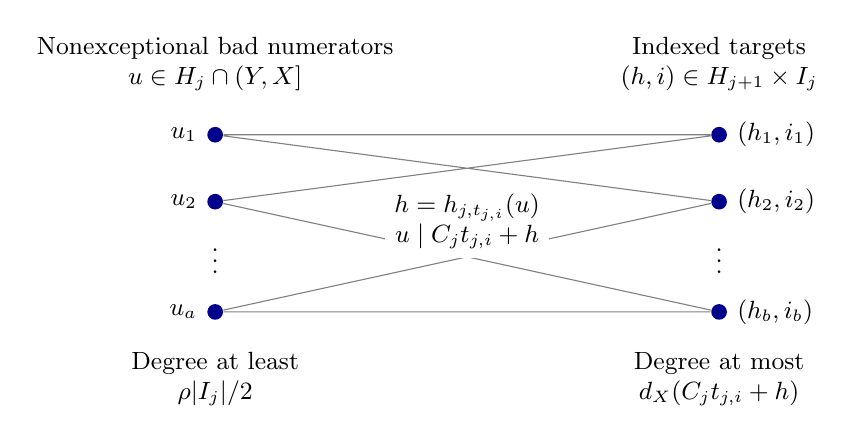
\begin{tikzpicture}[x=1cm,y=1cm,
  every node/.style={font=\small},
  point/.style={circle,fill=blue!55!black,inner sep=2pt}]
\node[align=center] at (0,1.15) {Nonexceptional bad numerators\\$u\in H_j\cap(Y,X]$};
\node[align=center] at (6.4,1.15) {Indexed targets\\$(h,i)\in H_{j+1}\times I_j$};
\node[point,label=left:$u_1$] (u1) at (0,0.25) {};
\node[point,label=left:$u_2$] (u2) at (0,-0.6) {};
\node at (0,-1.25) {$\vdots$};
\node[point,label=left:$u_a$] (ua) at (0,-2) {};
\node[point,label=right:{$(h_1,i_1)$}] (h1) at (6.4,0.25) {};
\node[point,label=right:{$(h_2,i_2)$}] (h2) at (6.4,-0.6) {};
\node at (6.4,-1.25) {$\vdots$};
\node[point,label=right:{$(h_b,i_b)$}] (hb) at (6.4,-2) {};
\draw[gray] (u1)--(h1) (u1)--(h2) (u2)--(h1) (u2)--(hb) (ua)--(h2) (ua)--(hb);
\node[fill=white,align=center] at (3.2,-0.85)
 {$h=h_{j,t_{j,i}}(u)$\\$u\mid C_jt_{j,i}+h$};
\node[align=center] at (0,-2.85) {Degree at least\\$\rho|I_j|/2$};
\node[align=center] at (6.4,-2.85) {Degree at most\\$d_X(C_jt_{j,i}+h)$};
\end{tikzpicture}
\caption{Schematic of the indexed predecessor count. Summing the right
 degrees and dividing by the left-degree lower bound gives the last term
 in \eqref{eq:bad-pair-count}. The Fourier-exception term
 $Xe^{-c_*m}$ and the inherited term $|H_{j+1}|$ are counted separately.
 Equal list values retain different indices. The drawn graph does not
 specify numerical degrees.}
\label{fig:predecessors}
\end{figure}

We check the hypotheses of Lemma~\ref{lem:divisor} before applying it.
Since \(j<d\), one has
\[
 \frac{S}{2\log S}\le m<\log X\le D_XS\le D_*S.
\]
Also
\[
 Y=Xe^{-\eta m}\ge X^{1-\eta}\ge\sqrt X,
 \qquad Y\le X.
\]
Finally, each shift \(N=C_jt_{j,i}\) is a positive integer and satisfies
\[
 N\le CM\le e^{(2D_C+D_M)S}<e^{D_*S}.
\]
Thus Lemma~\ref{lem:divisor}, with the fixed parameters \(D_*,r\),
applies uniformly at every level and to every list entry.
H\"older's inequality gives
\begin{align}
 \sum_{h\in H_{j+1}}d_X(N+h)
 &\le |H_{j+1}|^\alpha
       \left(\sum_{1\le h\le Y}d_X(N+h)^r\right)^{1/r}\notag\\
 &\le Y\,e^{S^{1/4}/r}\delta_{j+1}^{\alpha}.
 \label{eq:descent-holder}
\end{align}
This also holds when \(H_{j+1}\) is empty.
Substitution in \eqref{eq:bad-pair-count}, followed by division by \(X\),
uses \(Y=\rho X\) to cancel the factor \(1/\rho\):
\[
 \delta_j\le e^{-c_*m}+\rho\delta_{j+1}
                 +2e^{S^{1/4}/r}\delta_{j+1}^{\alpha}.
\]
Since \(\delta_{j+1}\le\delta_{j+1}^{\alpha}\), for sufficiently large
\(S\) we obtain the uniform recurrence
\begin{equation}\label{eq:density-recurrence}
 \delta_j\le\epsilon+A\delta_{j+1}^{\alpha},
 \qquad
 \epsilon=e^{-c_*m},\qquad A=e^{2S^{1/4}}.
\end{equation}

\paragraph{Iterating the recurrence.}
Our fixed choice of \(r\) ensures
\begin{equation}\label{eq:alpha-depth}
 \alpha^d
 \ge e^{-2d/r}
 \ge S^{-2K_d/r}
 \ge S^{-1/4},
\end{equation}
where we used \(-\log(1-1/r)\le2/r\) and
\eqref{eq:descent-depth}.
For nonnegative \(a,b\), the inequality
\((a+b)^\alpha\le a^\alpha+b^\alpha\) permits us to unroll
\eqref{eq:density-recurrence} from \(\delta_d=0\):
\begin{equation}\label{eq:density-unrolled}
 \delta_0\le
 \sum_{i=0}^{d-1}
 A^{(1-\alpha^i)/(1-\alpha)}\epsilon^{\alpha^i}
 \le d\exp\!\left(2rS^{1/4}-c_*mS^{-1/4}\right).
\end{equation}
Indeed, the exponent of \(A\) is at most \(r\), and
\(\alpha^i\ge\alpha^d\ge S^{-1/4}\).
The right-hand side tends to zero: the negative term has size at least
\(c_*S^{3/4}/(2\log S)\), which dominates the fixed multiple
\(2rS^{1/4}\) and \(\log d\).

For all sufficiently large \(S\), we therefore have
\[
 |H_0|\le X_0/8.
\]
Take \(G=G_0\) and \(X=X_0\).  By
\eqref{eq:descent-depth} and \eqref{eq:descent-length}, every \(u\in G\)
has an expansion of \(u/(MC)\) with at most
\((B_0+K_d)\log S\) terms.  The size bounds on \(M\) come from
Lemma~\ref{lem:residues}.  Every estimate above is uniform in the
allowed integer \(C\), and all thresholds depend only on fixed absolute
constants.  Choosing \(L=B_0+K_d\) and then one sufficiently large
absolute \(S_0\) proves Proposition~\ref{prop:density}.
\end{proof}

The proposition supplies short expansions on one common dense set of
numerators.  Section~\ref{sec:elementary} transfers this density statement
to every original fraction by writing a suitably scaled numerator as
the sum of two members of that set.

\section{Counting representations of one}\label{sec:counting}

We prove Corollary~\ref{cor:counting} using the uniform upper bound
in Theorem~\ref{thm:main}, together with the prime number theorem and
elementary identities. Divisor-rich denominators and divisor-indexed
splitting are also used by Konyagin and Elsholtz
\cite{Konyagin2014,Elsholtz2016}. The first step is
to obtain a short distinct expansion of one with a denominator having
many divisors. Lemma~\ref{lem:distinct} concerns totals below one; at
total one we need a different repetition-removal argument, preserving
an odd divisor of a denominator.

\begin{lemma}\label{lem:marked-cleanup}
Let $Q>1$ be odd. Suppose that a finite list of positive integers
$m_1,\ldots,m_t$ satisfies $\sum_{i=1}^t1/m_i=1$ and contains a
multiple of $Q$. Then $1$ has a representation by at most $t$ distinct
positive unit fractions, still with a denominator divisible by $Q$.
\end{lemma}

\begin{proof}
Whenever a denominator $m$ occurs twice, replace those two terms by
\[
 \frac2m=\frac1{m/2}\quad(m\text{ even}),
 \qquad
 \frac2m=\frac1{(m+1)/2}+\frac1{m(m+1)/2}
       \quad(m\text{ odd}).
\]
The sum stays equal to one and the length does not increase.
There remains a denominator divisible by $Q$: if no such denominator
is removed it persists, while if $Q\mid m$, the even replacement
$m/2$ is a multiple of $Q$ because $Q$ is odd, and the larger odd
replacement is a multiple of $m$.

This invariant excludes a denominator one, since that would force the
singleton list $(1)$. It also excludes a repeated denominator two,
since two halves exhaust the sum and neither denominator is divisible
by $Q$. Thus an odd repeated denominator is at least three. In an odd
replacement the smaller new denominator is strictly below $m$ and the
larger is strictly above $m$. The sorted denominator tuple therefore
strictly decreases lexicographically: all entries below $(m+1)/2$
are unchanged, and one extra copy of $(m+1)/2$ is inserted.
At a fixed length such a descent in positive integer tuples terminates.
Indeed, the first coordinate can decrease only finitely often, and
after it stabilizes the same argument applies successively to the other
coordinates. Even replacements strictly reduce length, so only finitely
many occur. The procedure consequently terminates with distinct
denominators and preserves the required multiple of $Q$.
\end{proof}

\begin{proof}[Proof of Corollary~\ref{cor:counting}]
\emph{A short initial expansion.}
Let $r$ be a sufficiently large integer and let $Q$ be the product of
the first $r$ odd primes. The prime number theorem, already used in
Section~\ref{sec:residues}, gives
\[
 \log Q=O(r\log r),\qquad \log\log Q=O(\log r).
\]
Apply Theorem~\ref{thm:main} to $(Q-1)/Q$ and append $1/Q$.
Lemma~\ref{lem:marked-cleanup} produces a distinct expansion of one
whose denominator set $S$ has size $s=O(\log r)$ and contains a
multiple $n$ of $Q$. Fix this one set $S$ and this one $n$.
Writing $\tau(n)$ for the number of positive divisors of $n$, we have
$\tau(n)\ge 2^r$.

\emph{Branching over divisors.}
For every positive proper divisor $d$ of $n$, the identity
\begin{equation}\label{eq:divisor-split}
 \frac1n=\frac1{n+d}+\frac1{n+n^2/d}
\end{equation}
gives two distinct integer denominators, with
\[
 n<n+d<2n<n+n^2/d.
\]
For each unchanged denominator in $S\setminus\{n\}$, at most one
choice of $d$ makes it equal to $n+d$, and at most one makes it equal
to $n+n^2/d$. Thus at least
\[
 \tau(n)-1-2(s-1)\ge 2^r-2s+1
\]
choices give distinct-denominator expansions of one, all of the same
length $\ell=s+1$. They give different expansions: from any resulting
denominator set, remove the fixed set $S\setminus\{n\}$; the smaller
of the two remaining denominators is $n+d$, which recovers $d$.
Sorting each set therefore gives a different tuple counted by $F(\ell)$.

\emph{Every sufficiently large length.}
For any distinct expansion of one with at least two terms, its largest
denominator $v$ exceeds one. Replace $v$ by $v+1$ and $v(v+1)$, using
\begin{equation}\label{eq:padding-split}
 \frac1v=\frac1{v+1}+\frac1{v(v+1)}.
\end{equation}
These are the two largest denominators of the new expansion. The
operation is injective: delete those two denominators and reinsert
the second largest minus one. Iterating a fixed number of times is
therefore injective. Our initial set contains a multiple of $Q>1$,
so it is not the singleton $\{1\}$; the operation applies to all
the expansions just constructed.

Choose an absolute constant $B\ge1$ such that $\ell\le B\log r$ for
all sufficiently large $r$. For each sufficiently large integer $k$,
take $r=\lfloor\exp(k/(2B))\rfloor$. Then $\ell\le k$, and applying
\eqref{eq:padding-split} exactly $k-\ell$ times to each of our
common-length expansions gives
\[
 F(k)\ge 2^r-2s+1\ge 2^{r-1}.
\]
Since $r\ge\tfrac12\exp(k/(2B))$ for large $k$, this proves
$\log\log F(k)\ge k/(2B)+O(1)$, hence the desired lower bound
for every sufficiently large integer $k$.

\emph{The upper bound.}
Fix a tuple counted by $F(k)$ and put $P_0=1$ and
$P_i=n_1\cdots n_i$. Before the $i$th term, the positive remainder
\[
 R_i=1-\sum_{j<i}\frac1{n_j}=\sum_{j=i}^k\frac1{n_j}
\]
is a rational number with a positive integer numerator over
$P_{i-1}$. Ordering therefore gives
\[
 \frac1{P_{i-1}}\le R_i\le\frac{k}{n_i},
 \qquad n_i\le kP_{i-1},\qquad P_i\le kP_{i-1}^2.
\]
Inductively $P_i\le k^{2^i-1}$ and $n_i\le k^{2^{i-1}}$.
Counting all integer choices in this larger box shows that $F(k)$ is
finite and
\[
 F(k)\le\prod_{i=1}^k k^{2^{i-1}}=k^{2^k-1}.
\]
Together with the lower bound, this yields
$\log\log F(k)\le k\log2+\log\log k=O(k)$ for sufficiently
large $k$, as required.
\end{proof}

\section{Preserving a prescribed denominator}\label{sec:prescribed}

Membership in $D_k$ requires the exact denominator $m$.
Lemma~\ref{lem:marked-cleanup}, used for counting, preserves only a
multiple of a specified odd integer, so it does not ensure that the
term $1/m$ survives. We instead reserve $1/m$ and use a greedy
construction that skips denominator $m$. It produces a distinct prefix
and makes the remaining sum smaller than every reserved reciprocal.
Any positive expansion of this remainder then avoids both the marker
and the prefix denominators.

We use this prefix twice: the uniform theorem first gives a short tail,
and a direct construction later gives the numerical bound in
Corollary~\ref{cor:prescribed}. Keeping the remainder unreduced retains
the divisors needed for that direct construction. In either case, a
separate padding argument will retain $m$ at every larger length.

\begin{lemma}[A greedy prefix avoiding one denominator]
\label{lem:marked-greedy-prefix}
Let $m\ge4$ and $T\ge2m^2$ be integers.
There are integers $2\le n_1<\cdots<n_j$, none equal to $m$,
and integers $q>0$ and $0\le R<2m$ such that
\[
  1=\frac1m+\sum_{i=1}^{j}\frac1{n_i}+\frac Rq,
  \qquad q=m\prod_{i=1}^{j}n_i,
  \qquad
  j<3+\log_2\log_2 T.
\]
Writing $q_0=m$ and $q_i=m\prod_{h=1}^{i}n_h$ for $1\le i\le j$,
we have $n_i\le q_{i-1}+1$ for every $1\le i\le j$.
If $R>0$, then
\[
  q\ge T,\qquad
  \frac Rq<\frac{2m}{T}\le\frac1m,
  \qquad \frac Rq<\frac1{n_i}\quad(1\le i\le j).
\]
In either case $q<T^2$.
\end{lemma}

\begin{proof}
Start with $(R_0,q_0)=(m-1,m)$ and $x_0=R_0/q_0$.
Whenever $R_i>0$ and $q_i<T$, set
\[
 a=\left\lceil\frac{q_i}{R_i}\right\rceil,
 \qquad
 n_{i+1}=\begin{cases}a,&a\ne m,\\m+1,&a=m,\end{cases}
 \qquad
 (R_{i+1},q_{i+1})=(n_{i+1}R_i-q_i,n_{i+1}q_i).
\]
Do not cancel common factors in this pair.  Thus
$x_{i+1}=R_{i+1}/q_{i+1}=x_i-1/n_{i+1}$.

For an ordinary step, writing $n=n_{i+1}=a$ gives
\[
  \frac1n\le x_i<\frac1{n-1},\qquad
  0\le R_{i+1}<R_i,\qquad
  0\le x_{i+1}<\frac1{n(n-1)}\le\frac1n.
\]
Moreover $n<1/x_i+1$, so
\[
 x_{i+1}<x_i-\frac{x_i}{1+x_i}
          =\frac{x_i^2}{1+x_i}<x_i^2.
\]
In the exceptional step $a=m$, we have
$(m-1)R_i<q_i\le mR_i$.  Consequently
\[
  0<R_i\le R_{i+1}<2R_i,
  \qquad
  0<x_{i+1}
   <\frac2{(m-1)(m+1)}<\frac1{m+1},
\]
where the last inequality uses $m\ge4$.
Every step therefore leaves a remainder smaller than the term just
subtracted.  The next denominator, if there is one, is strictly larger.
After the exceptional step all later denominators exceed $m+1$, so that
step can occur at most once.  Before it, $R_i\le m-1$; after it, the
numerator is less than $2(m-1)$ and decreases at every subsequent step.
Thus $0\le R_i<2m$ throughout.
Since $R_i\ge1$ in an active step, $a\le q_i$ and hence
$n_{i+1}\le q_i+1$.

All selected denominators are at least $2$, so $q_i$ at least doubles
at each step.  The procedure thus stops after finitely many steps.
Its first denominator is $2$, and
$x_1=(m-2)/(2m)<1/2$.
All later steps square the upper bound for the remainder, apart from
at most one step that still decreases it.  Therefore, whenever $i\ge2$
and the remainder is positive,
\[
 x_i\le 2^{-2^{i-2}},\qquad q_i\ge\frac1{x_i}
                 \ge2^{2^{i-2}}.
\]
If the final step has index $j\ge3$, its preceding state is active,
and hence
\[
 2^{2^{j-3}}\le q_{j-1}<T.
\]
This gives the asserted bound for $j$; it is immediate when $j\le2$.
The same preceding state satisfies
$q_j\le q_{j-1}(q_{j-1}+1)<T^2$, since $T$ is an integer.

The displayed decomposition and product formula follow by telescoping.
If $R_j=0$, the decomposition is complete.  Otherwise the stopping rule
gives $q_j\ge T$ and $R_j<2m$, whence
$R_j/q_j<2m/T\le1/m$.
At each earlier step the new remainder was smaller than $1/n_i$,
and subsequent steps only decrease it.  This proves all the claimed
strict inequalities.
\end{proof}

To see directly how the uniform theorem supplies a prescribed denominator,
take $T=2m^2$.  The lemma gives $j=O(\log\log m)$ and either a
complete marked expansion or a positive remainder $R/q$ with
\[
  1\le R<q,\qquad 2m^2\le q<4m^4.
\]
For sufficiently large $m$, the uniform upper bound in
Theorem~\ref{thm:main} applies to $R/q$, without requiring it to be
reduced.  It supplies a distinct expansion with
$O(\log\log q)=O(\log\log m)$ terms.  Each reciprocal in this
tail is at most its total $R/q$, which is strictly below $1/m$ and
every $1/n_i$.  The tail therefore avoids the marker and all prefix
denominators.  Together these terms give a distinct expansion of $1$
containing $1/m$, of length $O(\log\log m)$.

The same construction also supplies the finite exceptional values of
$m$, independently of the cutoff $T$.  For any fixed $m\ge4$, omit the condition
$q_i<T$ and continue until the remainder is zero.  The nonnegative
integer $R_i$ decreases strictly at every ordinary step, and there is
at most one exceptional step.  The process therefore terminates and
gives a distinct expansion of $1$ containing $1/m$.  For $m=2,3$, use
$1=1/2+1/3+1/6$.

The padding injection in Section~\ref{sec:counting} may remove the
denominator we wish to preserve. The following lemma supplies the
different property needed here: it increases the length and retains
any one prescribed denominator.

\begin{lemma}[Preserving a prescribed denominator while padding]
\label{lem:exact-marker-padding}
Let $r\ge3$ be an integer, and suppose that
\[
 1=\sum_{i=1}^{r}\frac1{n_i},\qquad
 1\le n_1<\cdots<n_r,
\]
where the denominators are integers. For every
$m\in\{n_1,\ldots,n_r\}$ there is a representation of $1$ by
exactly $r+1$ distinct positive unit fractions that still contains
the exact denominator $m$. Consequently $D_r\subseteq D_{r+1}$.
\end{lemma}

\begin{proof}
This is the padding lemma of van Doorn and Tang
\cite[Lemma~2.1]{vanDoornTang2026}; we include a proof.
Every denominator is at least two, since a term with denominator one
would already exhaust the sum. The identity
\[
 \frac1b=\frac1{b+1}+\frac1{b(b+1)}
\]
replaces one term by two with distinct denominators larger than $b$.
If $m\ne n_r$, apply it to $n_r$; the new denominators exceed all
the unchanged ones, and $m$ remains.

Suppose that $m=v=n_r$, and let $s=n_{r-1}$.
The same split of $s$ works unless $v=s+1$ or $v=s(s+1)$,
since every other unchanged denominator is smaller than $s$.
In either exceptional case, if $s=ab$ with integers $a,b\ge2$, use instead
\[
 \frac1s=\frac1{s+a}+\frac1{b(s+a)}.
\]
The inequalities
\[
 s+1<s+a<b(s+a)<s(s+1)
\]
show that both new denominators avoid either exceptional value of
$v$ and all the unchanged denominators below $s$.

Finally, neither exceptional case can occur when $s=p$ is prime.
There are at least three original terms, so $p>n_{r-2}\ge2$ and
in particular $p$ is odd. All denominators other than $p$ and $v$
are below $p$; write the sum of their reciprocals as $A/B$ with
$p\nmid B$. The two exceptional choices give respectively
\[
 1-\frac AB
 =\frac1p+\frac1{p+1}
 =\frac{2p+1}{p(p+1)},
 \qquad\text{or}\qquad
 1-\frac AB
 =\frac1p+\frac1{p(p+1)}
 =\frac{p+2}{p(p+1)}.
\]
After clearing denominators and reducing modulo $p$, these equations
give respectively $0\equiv B\pmod p$ and $0\equiv2B\pmod p$,
both impossible. Thus in every valid case an unmarked term can be
replaced by two distinct terms, preserving $m$ and increasing the
length by exactly one.
\end{proof}

\section{A quantitative prescribed-denominator bound}
\label{sec:prescribed-quantitative}

The uniform theorem gives the short marked expansion above with an
unspecified absolute length constant. We now prove the following
numerical estimate by constructing the tail directly.

\begin{proposition}\label{prop:marked-length}
For every $\varepsilon>0$ there is an integer $m_\varepsilon$ such
that every integer $m\ge m_\varepsilon$ occurs as an exact denominator
in a representation of $1$ by distinct positive unit fractions with
at most
\[
 \left(\frac{257}{\log 2}+\varepsilon\right)\log\log m
\]
terms.
\end{proposition}

The construction has two ingredients. A common integer $K_m$ supplies
short representations of small integers by positive rationals whose
numerators divide $K_m$. The unreduced denominator of the greedy
remainder has divisors at every multiplicative scale. Combining these
properties gives a short expansion of the tail: divisors of the greedy
denominator control how many pieces are needed, and the rational
representations supplied by $K_m$ bound the number of unit fractions
used for each piece.

\subsection{A common supply of rational divisors}

We construct a moderately sized integer whose divisors, after division by
positive integers, represent every integer in a prescribed initial interval
with a bounded number of summands.  The denominators of these rational
summands need not agree.  This freedom lets us first represent a positive
multiple of a prime and then divide by its integer multiplier.

\begin{lemma}\label{lem:rational-divisor-supply}
For every sufficiently large integer $m$, put
\[
 L=\log\log m,\qquad Y=m^4,\qquad
 \ell(v)=\left\lceil\frac{4\log v}{\log 2}\right\rceil
 \quad(v\geq2).
\]
Let $P(v)$ be the product of the first $\ell(v)$ primes, and define
\[
 K_m=P(Y)^2\,\lfloor L\rfloor!.
\]
Then $K_m>m$ and
\begin{equation}\label{eq:supply-size}
 \log K_m\leq
 \left(\frac{32}{\log 2}+o(1)\right)\log m\log\log m
 \qquad(m\longrightarrow\infty).
\end{equation}
Moreover, every integer $1\leq s\leq Y$ has a representation
\begin{equation}\label{eq:rational-supply}
 s=\sum_{i=1}^{h}\frac{e_i}{t_i},\qquad
 h\leq16,\quad e_i\mid K_m,\quad e_i,t_i\in\mathbb Z_{>0}.
\end{equation}
Repeated summands are allowed.
\end{lemma}

\begin{proof}
The prime number theorem \cite[p.~305, (1.1)]{Selberg1949} gives
\[
 \log P(v)=(1+o(1))\ell(v)\log\ell(v)
 \ll\log v\log\log v.
\]
Since $\ell(Y)=16\log m/\log 2+O(1)$, and
$\log(\lfloor L\rfloor!)=O(L\log L)$, this proves
\eqref{eq:supply-size}.  Also $P(Y)\geq2^{\ell(Y)}\geq Y^4$,
so $K_m>m$ for large $m$.

We next prove an assertion whose threshold is independent of $m$.
Fix a sufficiently large odd integer $u$, and let $A$ be the set of positive
divisors of $P(u)$.  Write $N=|A|=2^{\ell(u)}\geq u^4$.
We estimate exceptional primes by counting congruent pairs, the
mechanism underlying Gallagher's larger sieve \cite{Gallagher1971}.
The coarse count below suffices.
For each prime $p\leq u$, let $A_p$ be the image of $A$ in
$\mathbb F_p$.  Call $p$ exceptional when $|A_p|\leq p^{3/4}$.
If $c_a$ is the number of members of $A$ in residue class $a$, then
Cauchy--Schwarz shows that the number of ordered pairs of distinct members
of $A$ congruent modulo an exceptional prime is at least
\[
 \sum_{a\in\mathbb F_p}c_a^2-N
 \geq\frac{N^2}{|A_p|}-N
 \geq\frac{N^2}{2u^{3/4}}.
\]
For any two distinct members $a,b\in A$, the nonzero integer $|a-b|<P(u)$
has at most $\log P(u)/\log 2$ distinct prime divisors.
Counting the same pairs prime by prime therefore bounds the number $B(u)$
of exceptional primes by
\begin{equation}\label{eq:supply-exceptional}
 B(u)\leq \frac{2u^{3/4}\log P(u)}{\log 2}
 \ll u^{3/4}\log u\log\log u.
\end{equation}

We use the quantitative form of Vinogradov's three-prime theorem: there is
an absolute $c>0$ such that every sufficiently large odd integer $u$ has
at least $cu^2/(\log u)^3$ ordered representations as a sum of three
primes; see the statement in \cite[(1)--(2)]{Kumchev1997}
and the exposition in \cite[Theorem~1 and Section~3.1]{KumchevTolev2005}.
To make the uniformity in odd $u$ explicit, its singular series is
\[
 \mathfrak S(u)=
 \prod_{p\mid u}\left(1-\frac{1}{(p-1)^2}\right)
 \prod_{p\nmid u}\left(1+\frac{1}{(p-1)^3}\right).
\]
For odd $u$ its factor at $2$ is $2$, and
\[
 \mathfrak S(u)\geq
 2\prod_{p>2}\left(1-\frac{1}{(p-1)^2}\right)>0.
\]
The infinite product is positive because the sum of the subtracted
quantities converges.  Thus the asymptotic formula supplies an absolute
lower bound with an absolute threshold, with no dependence on the
factorization of $u$.

At most $3uB(u)$ ordered prime triples summing to $u$ contain an
exceptional prime: choose its position, its value, and one further entry;
the last entry is then fixed.  By \eqref{eq:supply-exceptional},
\[
 3uB(u)\ll u^{7/4}\log u\log\log u
       =o\left(\frac{u^2}{(\log u)^3}\right).
\]
Consequently every sufficiently large odd $u$ is the sum of three primes
that are not exceptional for this same set $A$.

It remains to represent each such prime using divisors of $P(u)^2$.
Fix one of them, say $p$, and put $H=A_p$ and $h=|H|>p^{3/4}$.
Let $U$ be the product of two independent uniformly chosen members of
$H$, and write $\mathrm e_p(z)=\exp(2\pi i z/p)$.
The following classical bilinear estimate is recorded in
\cite[Proposition~1.1]{GlibichukKonyagin2007}; we give its short proof
and the five-product consequence needed here.
For every nonzero $r\in\mathbb F_p$, orthogonality and
Cauchy--Schwarz give
\begin{align*}
 \left|\sum_{a,b\in H}\mathrm e_p(rab)\right|^2
 &\leq h\sum_{a\in\mathbb F_p}
       \left|\sum_{b\in H}\mathrm e_p(rab)\right|^2\\
 &=ph^2.
\end{align*}
After division by $h^4$, this says
\[
 \left|\mathbb E\,\mathrm e_p(rU)\right|
 \leq\frac{\sqrt p}{h}<p^{-1/4}.
\]
For five independent copies $U_1,\ldots,U_5$, Fourier inversion now yields
\begin{align*}
 \Pr(U_1+\cdots+U_5=0)
 &=\frac1p\left(1+\sum_{r\ne0}
                   (\mathbb E\,\mathrm e_p(rU))^5\right)\\
 &\geq\frac{1-(p-1)p^{-5/4}}p>0.
\end{align*}
Here the lower bound follows by bounding the absolute value of the sum
of the nonzero Fourier coefficients.

Choose pairs of residues witnessing this positive probability and lift
each residue to any positive member of $A$ representing it.  The five
integer products $e_1,\ldots,e_5$ are positive divisors of $P(u)^2$,
and their sum is divisible by $p$.  Hence
\[
 t=\frac{e_1+\cdots+e_5}{p}\in\mathbb Z_{>0},\qquad
 p=\sum_{i=1}^{5}\frac{e_i}{t}.
\]
The three chosen primes thus represent $u$ in fifteen summands of the
required kind.

For a sufficiently large integer $s$, use $u=s$ if $s$ is odd and
$u=s-1$ otherwise.  In the even case append the summand $1=1/1$.
This uses at most sixteen summands.  If $s\leq Y$, monotonicity of
$\ell$ implies $P(u)\mid P(Y)$, so every numerator constructed above
divides $K_m$.

Finally, all preceding thresholds concern $s$ alone and are absolute.
Choose an integer $S_0$ above them.  For all sufficiently large $m$ we
have $\lfloor L\rfloor\geq S_0$.  Each remaining integer
$1\leq s\leq S_0$ then divides $\lfloor L\rfloor!$ and hence $K_m$,
so it has the one-summand representation $s=s/1$.  This proves the
assertion simultaneously for every $1\leq s\leq Y$.
\end{proof}

\subsection{Grouping the remaining numerator}

The denominator retained by the greedy procedure has divisors at every
multiplicative scale.  We first record this property, then use it to reduce
the remaining numerator to a short list of integers within the range of
the rational-divisor supply.

\begin{lemma}\label{lem:marked-divisor-density}
Let $m\ge2$ be an integer.  Suppose that $q$ is obtained from $m$ by a
finite sequence of replacements $q\mapsto nq$, where at each replacement
$n$ is a positive integer satisfying $n\le q+1$.  Then, for every real
number $w$ with $1\le w\le q$, there is a positive divisor $d$ of $q$ such
that
\[
  \frac wm\le d\le w.
\]
\end{lemma}

\begin{proof}
For the initial value $q=m$, the divisor $1$ works throughout $[1,m]$.
Suppose the property holds for $q$, and put $q'=nq$.  If $1\le w\le q$,
use a divisor of $q$, which is also a divisor of $q'$.  If $n\le w\le nq$,
apply the property at $w/n$ and multiply the resulting divisor by $n$.
These two cases cover $[1,nq]$ unless $q<n$ and $q<w<n$.  In that gap
the divisor $q$ itself works: $q<w$ and
\[
  w<n\le q+1\le mq.
\]
This proves the induction, including the real points between consecutive
integers.
\end{proof}

\begin{lemma}\label{lem:marked-grouping}
Let $m\ge2$, $q\ge1$, $K_m\ge1$, and $B\ge1$ be integers.  Suppose that, for every
real $w\in[1,q]$, the integer $q$ has a divisor in $[w/m,w]$.  Suppose
also that each integer $s\in[1,m^4]$ can be written as a sum of at most
$B$ positive rational numbers $e/t$, where $e\mid K_m$ and $t$ is a
positive integer.  Then, for every integer $X$ with $1\le X\le q$, the
rational number $X/(qK_m)$ is a sum of at most
\[
  B\left(\frac{\log X}{2\log m}+2\right)
\]
positive unit fractions, with repetitions allowed.
\end{lemma}

\begin{proof}
Write $X_0=X$, and repeatedly remove groups from the remaining integer.
If the current integer $X_i$ exceeds $m^4$, then
$w=X_i/m^2$ lies in $[1,q]$.  Choose $d_i\mid q$ with
\[
  \frac{X_i}{m^3}\le d_i\le\frac{X_i}{m^2},
  \qquad s_i=\left\lfloor\frac{X_i}{d_i}\right\rfloor.
\]
Thus $m^2\le s_i\le m^3\le m^4$, and the integer remaining after the
group $d_i s_i$ is removed satisfies
\[
  0\le X_{i+1}=X_i-d_i s_i<d_i\le\frac{X_i}{m^2}.
\]
If instead $0<X_i\le m^4$, remove the final group with $d_i=1$ and
$s_i=X_i$.  Stop immediately if the remaining integer is zero.

Every grouping step with $X_i>m^4$ decreases the remainder by a factor
strictly greater than $m^2$.  There are therefore at most
$\lceil\log X/(2\log m)\rceil$ such steps, followed by at most one
final group.  The number $G$ of groups satisfies
\[
  G\le\left\lceil\frac{\log X}{2\log m}\right\rceil+1
    \le\frac{\log X}{2\log m}+2.
\]
This bound also covers $X=1$ and a zero remainder before the final group.

For each group, use the assumed representation
$s_i=\sum_{a=1}^{b_i}e_{i,a}/t_{i,a}$, with $b_i\le B$.
Dividing $X=\sum_i d_i s_i$ by $qK_m$ gives
\[
  \frac{X}{qK_m}
    =\sum_i\sum_{a=1}^{b_i}
       \frac{1}{(q/d_i)(K_m/e_{i,a})t_{i,a}}.
\]
Each displayed denominator is a positive integer.  This uses the two
divisibilities $d_i\mid q$ and $e_{i,a}\mid K_m$; no divisibility between
$t_{i,a}$ and $e_{i,a}$, or coprimality assumption, is needed.  The total
number of terms is at most $BG$.
\end{proof}

\begin{proof}[Proof of Proposition~\ref{prop:marked-length}]
Fix a sufficiently large integer $m$, put $L=\log\log m$, and take
$K_m$ from Lemma~\ref{lem:rational-divisor-supply}. Apply
Lemma~\ref{lem:marked-greedy-prefix} with $T=2mK_m$, which is an
integer at least $2m^2$. It gives
\[
 1=\frac1m+\sum_{i=1}^{j}\frac1{n_i}+\frac Rq,
 \qquad 0\le R<2m.
\]
The prefix is distinct and avoids $m$. By \eqref{eq:supply-size},
\[
 \log\log(2mK_m)\le L+O(\log L),
 \qquad
 j\le\frac{L}{\log2}+O(\log L)
   =\left(\frac1{\log2}+o(1)\right)L.
\]
If $R=0$, the expansion is complete and already satisfies the asserted
length bound. Suppose henceforth that $R>0$.

The denominator $q$ is retained without cancellation, beginning at $m$
and using multipliers at most the preceding denominator plus one.
Lemma~\ref{lem:marked-divisor-density} therefore applies to this $q$.
Moreover $q\ge2mK_m$ and $R<2m$, so the integer $X=RK_m$ satisfies
$1\le X<q$. Lemma~\ref{lem:marked-grouping}, with $B=16$ and the
supply from Lemma~\ref{lem:rational-divisor-supply}, represents
$X/(qK_m)=R/q$ as a sum of at most $16G$ unit fractions, where
\[
 G\le\frac{\log(RK_m)}{2\log m}+2
 \le\frac{\log K_m+\log(2m)}{2\log m}+2
 \le\left(\frac{16}{\log2}+o(1)\right)L.
\]
This count depends on $RK_m$, not on the potentially much larger $q$.

Apply Lemma~\ref{lem:distinct} only to this tail. It makes its
denominators distinct without changing its number of terms. The tail
sum is strictly below $1/m$ and every $1/n_i$ by
Lemma~\ref{lem:marked-greedy-prefix}. Every reciprocal in any positive
expansion of that sum is at most the sum itself. Thus all denominators
of the distinct tail exceed $m$ and every $n_i$, so adjoining it to the
reserved term and prefix produces a distinct expansion of $1$.
There is one reserved term, $j$ prefix terms, and at most sixteen terms
for each of the $G$ groups. Its total length is therefore at most
\[
 1+j+16G
 \le\left(\frac{1+16\cdot16}{\log2}+o(1)\right)L
 =\left(\frac{257}{\log2}+o(1)\right)\log\log m.
\]
All errors here tend to zero as $m$ tends to infinity through all
integers: the bound on $R$ removed any dependence on the chosen
stopping numerator, and the supply covers both parities. Absorbing
the error into any prescribed $\varepsilon>0$ proves the proposition.
\end{proof}

\subsection{Every sufficiently large prescribed length}

\begin{proof}[Proof of Corollary~\ref{cor:prescribed}]
Set $A=257/\log2$. Fix a real number $c$ with $0<c<1/A$, and
choose $\varepsilon>0$ such that $c(A+\varepsilon)<1$.
Proposition~\ref{prop:marked-length} supplies an integer $M\ge4$ such
that every integer $m\ge M$ has a distinct marked expansion with
at most $(A+\varepsilon)\log\log m$ terms. The construction in
Section~\ref{sec:prescribed} also gives a finite distinct marked
expansion for each $2\le m<M$. Fix one for each such $m$, and let
$k_*$ be the maximum of their finitely many lengths.

For every integer $k\ge k_*$ and every integer
$2\le m\le\exp(\exp(ck))$, the chosen expansion has at most $k$
terms. This is immediate for $m<M$; for $m\ge M$ its length is at
most
\[
 (A+\varepsilon)\log\log m
 \le c(A+\varepsilon)k<k.
\]
A distinct expansion of $1$ containing a denominator $m\ge2$ has
at least three terms: denominator one would exhaust the sum, and two
distinct denominators at least two contribute at most $1/2+1/3<1$.
Thus Lemma~\ref{lem:exact-marker-padding} may be iterated until the
length is exactly $k$, retaining the exact integer $m$. We have proved
\[
 \{2,\ldots,\lfloor\exp(\exp(ck))\rfloor\}\subseteq D_k.
\]
The first missing integer exceeds the real right endpoint, and hence
$v(k)\ge\exp(\exp(ck))$ for every sufficiently large integer $k$.
Because this holds for each fixed $c<\log2/257$, it gives
\[
 \liminf_{k\to\infty}\frac{\log\log v(k)}{k}
 \ge\frac{\log2}{257}.
\]
In particular $257/\log2<600$, so taking $c=1/600$ gives the stated
eventual lower bound $v(k)\ge\exp(\exp(k/600))$.

For the upper bound, the product recurrence in the proof of
Corollary~\ref{cor:counting} gives $n_i\le k^{2^{i-1}}$ in every
distinct exact-$k$ expansion of $1$. Every denominator in such an
expansion is therefore at most $k^{2^{k-1}}$. Consequently $D_k$ is
finite for every $k\ge1$, its complement in $\{2,3,\ldots\}$ is
nonempty, and
\[
 v(k)\le1+k^{2^{k-1}}.
\]
For $k\ge2$ this yields
$\log\log v(k)\le k\log2+\log\log k$, and therefore
\[
 \limsup_{k\to\infty}\frac{\log\log v(k)}{k}\le\log2.
\]
Together the two bounds imply $\log\log v(k)=\Theta(k)$.
\end{proof}

The lower slope above is the consequence of the length coefficient
in Proposition~\ref{prop:marked-length}. Its vanishing error does not
imply an eventual inequality with the endpoint $c=\log2/257$.
Neither that endpoint inequality nor a limiting or sharp slope is
asserted.


\begingroup
\small
\bibliographystyle{plain}
\bibliography{references}
\endgroup
\end{document}
